\documentclass{beamer}
\usepackage{pgfpages}

\setbeamertemplate{note page}[plain]
\setbeameroption{show notes on second screen=bottom}
% \setbeameroption{show notes on second screen=right}
\usetheme{Madrid}
\beamertemplatenavigationsymbolsempty

\usepackage[utf8]{inputenc}
% font - Palatino
\usepackage[sc,osf]{mathpazo}   % With old-style figures and real smallcaps.
\usepackage[euler-digits,small]{eulervm}
\usepackage[style=authortitle-comp, backend=biber]{biblatex}
\usepackage{xpatch}
\xapptobibmacro{cite}{\setunit{\nametitledelim}\printfield{year}}{}{}
\addbibresource{./references.bib}
\usepackage[compat=1.1.0]{tikz-feynman}
\usepackage{bm}
\usepackage{commath}
\usepackage{booktabs} % \toprule, \midrule
\usepackage{multirow} % \multirow
\usepackage{tabularx}
\usepackage{colortbl} % \rowcolor in tables
\usepackage{adjustbox} % \resizebox for table
\usepackage{xcolor}
\usepackage{caption}
\usepackage{siunitx}
\usepackage{appendixnumberbeamer}
\usepackage{booktabs} % \toprule etc.
\usepackage{nccmath} % center equation
\usepackage{tikz}
\usetikzlibrary{positioning}
\usetikzlibrary{arrows}


\DeclareMathOperator{\Ima}{Im}
\DeclareMathOperator{\sfm2}{sfm2}
\DeclareMathOperator{\cov}{cov}
\DeclareMathOperator{\dim}{dim}

\definecolor{primary}{rgb}{0.78, 0.89, 1}
\setbeamercolor{palette primary}{fg=white,bg=black!80}
\setbeamercolor{palette secondary}{fg=white,bg=black!40}
\setbeamercolor{palette tertiary}{fg=black,bg=black!20}
\setbeamercolor{caption name}{fg=black}
\setbeamercolor{block title}{bg=black!40}

\setbeamertemplate{section in toc}{ {\color{black}\inserttocsectionnumber.~\inserttocsection} }
\setbeamertemplate{subsection in toc}{ \hspace{1.2em}{\color{black}\rule[0.3ex]{3pt}{3pt}}~\inserttocsubsection\par }
\setbeamertemplate{subsubsection in toc}{ \hspace{2.4em}{\color{black}\rule[0.2ex]{2pt}{2pt}}~\inserttocsubsubsection\par }
\setbeamertemplate{itemize items}{\scriptsize\color{black!70}\(\blacksquare\)}

\setbeamertemplate{blocks}[default]
\setbeamerfont{caption}{size=\tiny}

\setbeamerfont{myTOC}{size=\normalsize}
\AtBeginSection[]{
  \ifnum \value{framenumber}>1
    \frame{\frametitle{Table of Contents}\usebeamerfont{myTOC}\tableofcontents[current]}

  \else
  \fi
}

% Custom Footer
\makeatletter
\setbeamertemplate{footline}
{
  \leavevmode%
  \hbox{%
    \begin{beamercolorbox}[wd=.333333\paperwidth,ht=2.25ex,dp=1ex,center]{author in head/foot}%
      \usebeamerfont{author in head/foot}\insertsection
    \end{beamercolorbox}%
    \begin{beamercolorbox}[wd=.333333\paperwidth,ht=2.25ex,dp=1ex,center]{title in head/foot}%
      \usebeamerfont{title in head/foot}\insertsubsection
    \end{beamercolorbox}%
    \begin{beamercolorbox}[wd=.333333\paperwidth,ht=2.25ex,dp=1ex,right]{date in head/foot}%
      \usebeamerfont{date in head/foot}\insertshortdate{}\hspace*{2em}
      \insertframenumber{} / \inserttotalframenumber\hspace*{2ex} 
    \end{beamercolorbox}}%
  \vskip0pt%
}
\makeatother


\title[The Strong Coupling]{The QCD Strong Coupling from Hadronic Tau Decays}
% \subtitle{A PhD Defense}
\author{\Large Dirk Hornung}
\institute{
  \normalsize
  \textsc{Supervisor} \\
  Matthias Jamin
}
\titlegraphic{
  \includegraphics[height=1.5cm]{./images/logo_uab.eps}
  \hspace{5cm}
  \includegraphics[height=1.5cm]{./images/logo_ifae.eps}
}
\date{17th July 2019}


\begin{document}
\frame{\titlepage}

\section{Introduction}
\begin{frame}
  \frametitle{The Running of the Strong Coupling}
  \begin{itemize}
  \item The strong coupling depends on energy
    \begin{columns}
      \begin{column}{0.35\textwidth}
        \begin{equation}
          \begin{split}
            \alpha_s(m_\tau^2) &\approx 0.33 \\
            \alpha_s(m_Z^2) &\approx  0.12
          \end{split}
        \end{equation}
        \begin{footnotesize}
          \begin{equation}
            \begin{split}
              m_\tau &= \SI{1776.86 \pm 0.12}{\mega\eV}\footnotemark \\
              m_Z &= \SI{91.1876 \pm 0.0021}{\giga\eV}^1
            \end{split}
          \end{equation}
        \end{footnotesize}
      \end{column}
      \begin{column}{0.65\textwidth}
        \begin{figure}
          \vspace{0.5cm}
          \includegraphics[width=\textwidth]{./images/runningOfAs.eps}\\[-1ex]
          \captionsetup{format=hang}
          \caption{\tiny Taken from \cite{PDG2018}}
        \end{figure}
      \end{column}
    \end{columns}
    \footnotetext{\cite{PDG2018}}
  \end{itemize}
\end{frame}
\note[itemize]{
  \item \(\alpha_s\) depends on energy 
  \item Referred to as ``running of the strong coupling''
  \item E.g. \(\alpha_s(m_\tau^2) \approx 0.33\)
  \item Compare at \(m_Z^2\) scale
  \item Plot which shows the running of \(\alpha_s\)
  \item \(\alpha_s\) decreases with increasing energy
  \item Asymptotic freedom: at high energies quarks and gluons interact
    weakly
  \item Confinement: at low energies quarks are bound. An isolated
    quark has never been measured. They appear as hadrons.
  \item for \(\alpha_s > 0.5\) PT breaks down
  \item Hadronic tau decays good for measuring \(\alpha_s\)
    \begin{itemize}
      \item \(\alpha\) small enough for PT
      \item \(\alpha\) large enough to be sensitive
    \end{itemize}
  \item Errors also decrease with energy
  \item Tau decays extract \(\alpha_s\) at low energies as compared to other methods
}

\begin{frame}
  \frametitle{Tau decays}
  \begin{itemize}
  \item Feynman diagram of the tau decay
    \begin{center}
      \feynmandiagram [scale=0.8, layered layout, horizontal=a to b] {
        a [particle=\(\tau^{-}\)] -- [fermion] b -- [fermion] f1 [particle=\(\nu_{\tau}\)], b -- [boson, edge label'=\(W^{-}\)] c,
        c -- [anti fermion] f2 [particle={\footnotesize\(e^-, \mu^-,
          \overline{u}, \overline{u} \)}],
        c -- [fermion] f3 [particle={\footnotesize\(\overline{\nu}_e,
          \overline{\nu}_\mu, d, s\)}],
      };
    \end{center}
  \item Mesons produced by tau decays
    \begin{footnotesize}
      \begin{center}
        \begin{tabular}{ccc}
          \toprule
          Symbol & Quark content & Rest mass \\
          \midrule
          \(\pi^-\) & \(\overline{u} d\) & \SI{139.57061 \pm 0.00024}{\mega\eV}  \\
          \(\pi^0\) & \((u \overline{u} - d \overline{d})/\sqrt{2}\) & \SI{134.9770\pm0.0005}{\mega\eV} \\
          \(K^-\) & \(\overline{u} s\) & \SI{493.677\pm0.016}{\mega\eV} \\
          \(K^0\) & \(d \overline{s}\) & \SI{497.611\pm0.013}{\mega\eV}
        \end{tabular}
      \end{center}
      \begin{equation}
        \mathcal{B}(\tau \to \pi^- \nu_\tau) &= 10.81\%, \quad \mathcal{B}(\tau \to K^-) &= 0.70\%
      \end{equation}
    \end{footnotesize}
  \end{itemize}
\end{frame}
\note[itemize]{
  \item \(\alpha_s\) from hadronic tau decays
  \item Described by Feynman Diagram
    \begin{itemize}
    \item Tau decay into \(W\) boson and \(\nu_\tau\)
    \item \(W\) decays into \(e^-, \mu^-\) and their corresponding neutrinos or
      \(u, d\) or \(s\) quarks
    \item only lepton decaying into quarks
    \end{itemize}
  \item Confinement: Don't measure quarks but hadrons
  \item Hadrons: Composite particles that consist of quarks
  \item We have to apply Duality to match QCD calculations with experiment
  \item Produced meson table: pion, kaon
  \item \(\tau \to \pi^-\nu_\tau\) Cabbibo allowed, \(\tau \to K^- \nu_\tau\) Cabbibo suppressed (\(\abs{V_{us}}^2 = (0.2)^2\))
  \item will focus non-strange tau decays, (only \(u, d\) quarks)
}

\begin{frame}
  \frametitle{Table of Contents}
  \tableofcontents[subsubsectionstyle=hide]
\end{frame} 

\section{Theoretical Framework}
\begin{frame}
  \frametitle{Two-Point Function}
  \begin{block}{Two-Point Function:}
    \begin{equation}
      \begin{split}
        \Pi_{V/A}^{\mu\nu}(q^2) &\equiv i \int \dif^4 x e^{iqx} \langle 0\vert T \left\{ J_{V/A}^\mu(x) J_{V/A}^\nu(0)\right\} \vert 0 \rangle \\
        &= (q^\mu q^\nu - q^2 g^{\mu\nu})\Pi_{V/A}^{(1)}(q^2) + q^\mu q^\nu
        \Pi_{V/A}^{(0)}(q^2)
      \end{split}
    \end{equation}
  \end{block}
  \small where the current is given by
  \begin{equation*}
    J_V^\mu = \overline{u} \gamma^\mu d\) \quad \text{and} \quad \(J_A^\mu = \overline{u} \gamma^\mu \gamma_5 d
  \end{equation*}
\end{frame}
\note[itemize] {
\item Two-point function is the vacuum expectation value of the time-ordered
  product of two currents
\item Non-strange \(V\) or \(A\) currents, distinguished by a \(\gamma^\mu\) or
  \(\gamma^\mu\gamma_5\)
\item Lorentz decompose to obtain a scalar functions \(\Pi\) of different spin
  \((0)\) and \((1)\)
\item Two-point function has poles on the positive real axis, but elsewhere analytic
}

\begin{frame}
  \frametitle{Cauchy's Theorem}
  \centering
  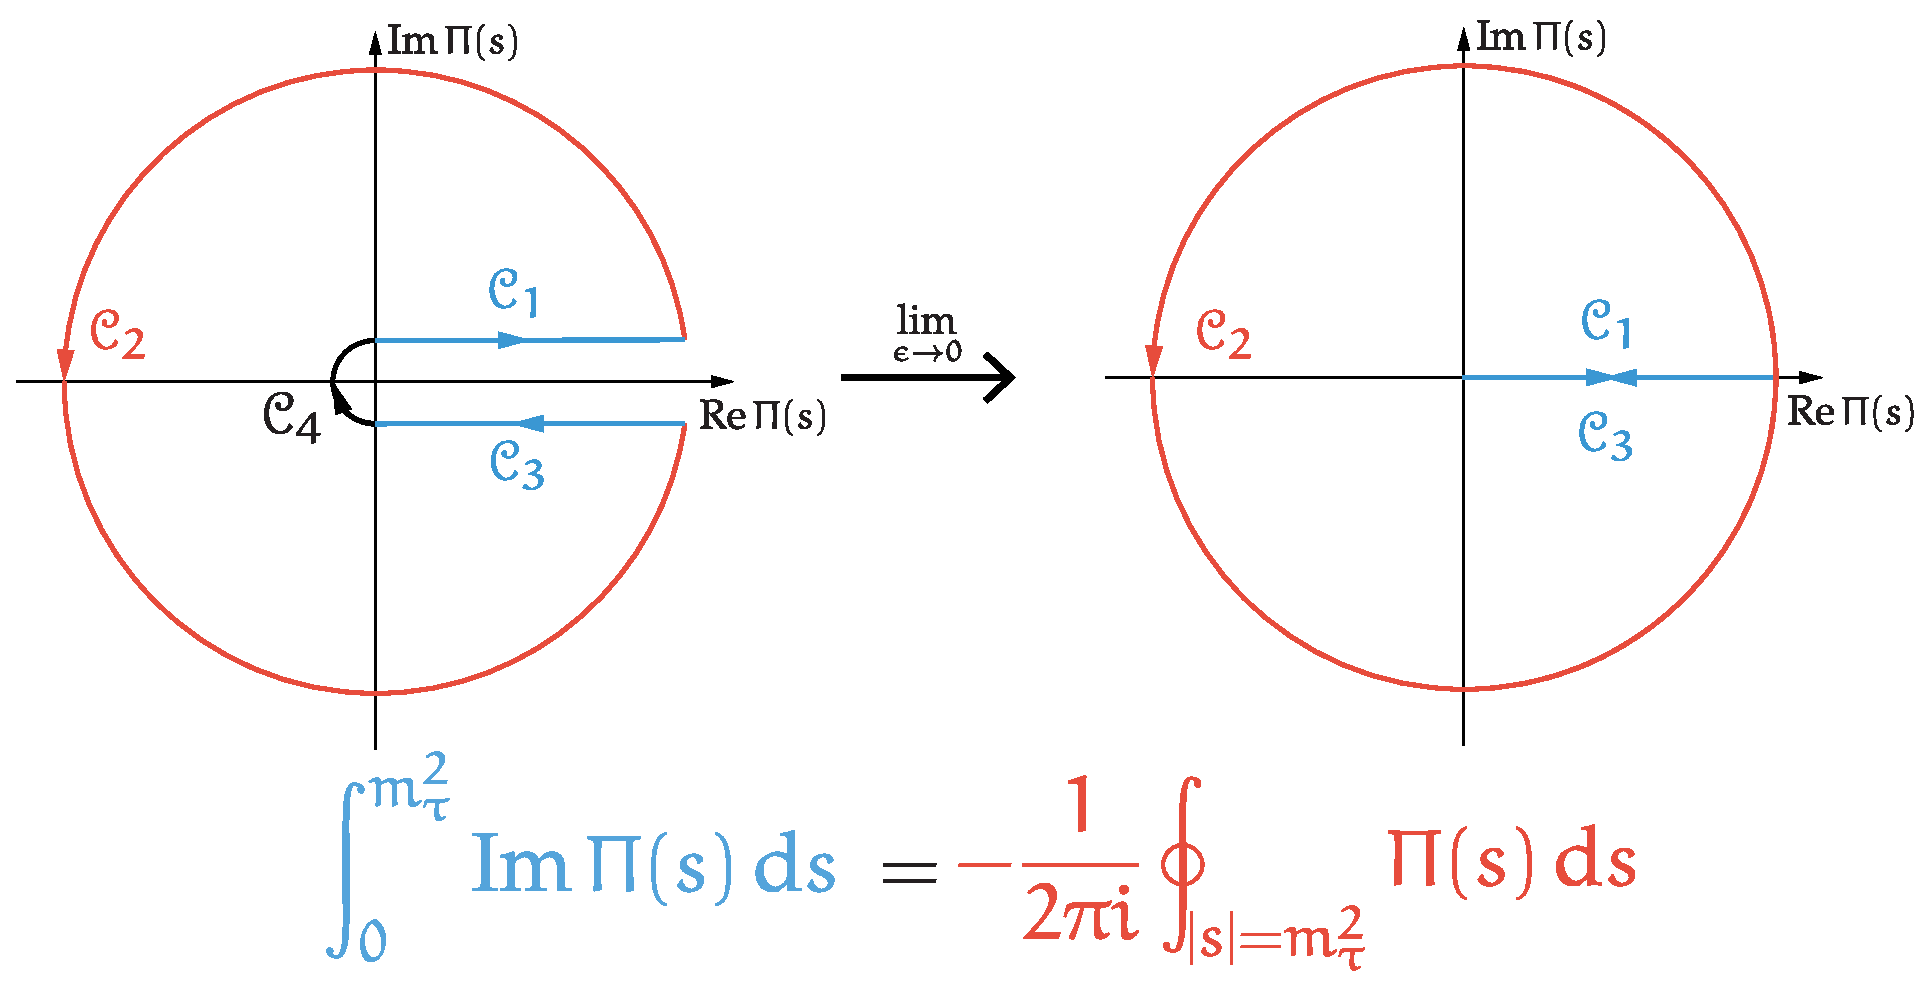
\includegraphics[width=0.6\textwidth]{./images/rTauCauchysTheorem.eps}
\end{frame}
\note[itemize]{
\item Avoid to calculate correlator close to the positive real axis,
\item Calculate correlator at large \(s\)
\item Closed contour integral over an analytic function is zero
\item Construct closed contour integral
\item Red is the outer circle, which will be calculated theoretically
\item Blue line integral experimentally accessible
\item \(\epsilon\) is the radius of the inner circle
\item If we take the limit of \(\epsilon \to 0\) the red circle is equal the
  blue line
\item The contributions of the correlator close to positive real axis will be
  suppressed by weights
\item \(\mathcal{C}_4\) vanishes due to no physical contributions!
}

\begin{frame}
  \frametitle{Finite Energy Sum Rules}
  \begin{itemize}
  \item Spectral Function:
    \begin{equation}
      \rho(s) = \frac{1}{\pi} \Ima \Pi(s)
    \end{equation}
    \begin{block}{Integral Moment}
      \begin{equation}
        I_{V/A}^{(\omega)}(s_0) \equiv \frac{12 \pi^2}{s_0} \int_0^{s_0} \dif s \omega\, \left(\frac{s}{s_0}\right) \rho^{exp}_{V/A}(s)
        = \frac{6 \pi i}{s_0} \oint_{\abs{s}=s_0} \dif s\, \omega\left(\frac{s}{s_0}\right) \Pi^{th}_{V/A}(s)
      \end{equation}
    \end{block}
    \item The lhs is given by experiment, the rhs is theoretically calculated.
  \end{itemize}
\end{frame}
\note[itemize]{
\item Experimental data given in form of spectral function
\item Connect the experiment with theory via integral moment
\item Define the experimental integral moment, introducing a weight \(\omega\)
\item Applied Cauchy's theorem to get theoretical integral moment
\item Note: Moments depend on \(\omega\) and \(s_0\)
\item Will construct chi-squared from moments
}

\subsection{Theoretical Computation}
\begin{frame}
  \centering \vspace{0.5cm}
  \begin{LARGE}
    The Theoretical Computation
  \end{LARGE}
  \begin{equation}
    I^{th}(s_0) \equiv - \frac{1}{2 \pi i s_0} \oint_{\abs{s}=s_0} \dif s \omega\left(\frac{s}{s_0}\right) \Pi_{V/A}^{th}(s)
  \end{equation}
\end{frame}

\begin{frame}
  \frametitle{Operator Product Expansion}
  \begin{itemize}
  \item The correlator is approximated by the operator product expansion
    \begin{equation}
      \Pi^{th} \to \Pi^{OPE}(s) = \sum_D \frac{1}{(s)^{D/2}} \sum_{\dim \mathcal{O} = D} C_{D}(s,\mu)\langle \mathcal{O}(\mu) \rangle
      \equiv \sum_{k=0}^\infty \frac{C_{2k}(s)}{(s)^k}
    \end{equation}
  \item \(C_{D}\) are the Wilson coefficients, which can be calculated
    perturbatively
  \item \(\mathcal{O}\) are higher dimensional operators, e.g. \(D=4\)
    \begin{itemize}
    \item Quark condensate: \(m\langle \overline{q}{q} \rangle\)
    \item Gluon condensate: \(\langle G_a^{\mu\nu}G^{a}_{\mu\nu} \rangle\)
    \end{itemize}
  \item The term with \(D = 0\) corresponds to the perturbative contribution
  \item In approximating \(\Pi^{th} \to \Pi^{OPE}\) we assume Duality
  \end{itemize}
\end{frame}
\note[itemize]{
\item QCD vacuum cannot be solely described by PT methods
\item Approximate correlator with OPE
\item The OPE separates short distances (high energies/ PT) from long distances
  (NPT)
\item Short distances \(\Rightarrow\) Wilson coefficients calculated by Feynman
  diagrams
\item Long distances \(\Rightarrow\) vacuum expectation value of higher
  dimensional operators
\item E.g. \(D=4\) are the quark condensate and gluon condensate
\item Have to be obtained by NPT methods like lattice QCD or from our fits
\item Will fit up to dimension 12
\item The term \(D=0\) corresponds to PT
\item In approximating the correlator with the OPE we assume quark-hadron
  duality }

\begin{frame}
  \frametitle{Quark-Hadron Duality}
  \begin{itemize}
  \item The equality of the quark-gluon picture and the hadronic picture is
    called quark-hadron duality
  \item Differences between the physical spectral function and its OPE
    approximation are referred to as duality violations
  \item DV can be modelled with the following ansatz:
    \begin{equation}
      \rho_{V/A}^{DV}(s) = e^{-(\delta_{V/A} + \gamma_{V/A}s)} \sin(\alpha_{V/A} + \beta_{V/A}s)
    \end{equation}
    \begin{scriptsize}
      \cite{Boito2011a}
    \end{scriptsize}
  \item The Model is theoretically well motivated, but cannot be derived from
    first principles
  \end{itemize}
\end{frame}
\note[itemize]{
\item Theoretically work in quark-gluon picture, experimentally observe hadrons
  \(\Rightarrow\) quark-hadron duality
\item The physical spectral function differs from its OPE approximation
  \(\Rightarrow\) Duality Violations
\item DV can be parametrised via a model
\item Theoretically well motivated but cannot be derived from first principles
\item Four parameters V + four parameters A
\item Too many parameters: e.g. \(\alpha_s, \rho_6, \rho_8\) three parameters vs
  eight!
\item We investigate contribution of DV, if sufficient suppressed }

\begin{frame}
  \frametitle{Perturbative Contribution}
  \begin{itemize}
  \item In the chiral limit the vector and axial-vector contributions are equal
  \item The renormalisation-scale-invariant Adler function:
    \begin{equation}
      D_{OPE}^{D=0}(s) \equiv -s \frac{\dif}{\dif s} \Pi(s)
      = \frac{1}{4 \pi^2} \sum_{n=0}^\infty a^n(\mu^2) \sum_{k=1}^{n+1} k\, c_{n,k} \log\left( \frac{-s}{\mu^2} \right)^{k-1}
    \end{equation}
    where
    \begin{equation}
      a(\mu^2) \equiv \frac{\alpha_s(\mu^2)}{\pi}
    \end{equation}
  \item The Adler function only depends on the coefficients \(c_{n,1}\). All
    other \(c_{n,k}\) can be expressed in terms of the \(c_{n,1}\) through the
    RGE.
    \begin{equation}
      \begin{split}
        c_{0,1} = c_{1,1} = 1, \quad c_{2,1} = 1.63982, \quad c_{3,1} = 6.37101 \\
        c_{4,1} = 49.07570 \quad c_{5,1} = 283 \pm 283\, \text{(estimate)}
      \end{split}
    \end{equation}
  \end{itemize}
\end{frame}
\note[itemize]{
\item Work in chiral limit: V and A contributions are equal
\item Contour integral can be expressed by Adler function
\item In case of vector correlator the derivative (Adler Function) is a physical
  quantity.
\item Physical quantities are renormalisation scale invariant.
\item Depends on Adler function coefficients, which can be calculated from
  Feynman diagrams
\item Only have to calculate \(c_{n,1}\) coefficients, rest are mapped via RGE
}

\begin{frame}
  \frametitle{Perturbative Contribution}
  \begin{itemize}
  \item Perturbative Integral Moment:
    \begin{equation}
      \begin{split}
        I^{th,PT} &\equiv \frac{6 \pi i}{s_0} \oint_{\abs{s}=s_0} \dif s\, \omega\left(\frac{s}{s_0}\right) \Pi_{OPE}^{D=0}(s) \\
        &= -\frac{3 \pi i}{s_0} \oint_{\abs{s}=s_0} \frac{\dif s}{s} \omega_D\left(\frac{s}{s_0}\right) D_{OPE}^{D=0}(s) \\
        &= -\frac{3 i}{4 \pi s_0} \oint_{\abs{s}=s_0} \frac{\dif s}{s}
        \omega_D\left(\frac{s}{s_0}\right) \sum_{n=0}^\infty a^n(\mu^2)
        \sum_{k=1}^{n+1} k\, c_{n,k} \log\left( \frac{-s}{\mu^2} \right)^{k-1}
      \end{split}
    \end{equation}
    where
    \begin{equation}
      \omega_D \equiv 2 \int_{s/s_0}^{1} \omega\left( \frac{s^\prime}{s_0} \right) \dif s
    \end{equation}
  \item E.g. kinematic weight
    \begin{equation}
      \omega_\tau(s) \equiv \left(1 - \frac{s}{s_0}\right)^2\left( 1 + 2 \frac{s}{s_0} \right)
      \, \Rightarrow \,
      \omega_{D, \tau}(s) = -\left(1-\frac{s}{s_0}\right)^3 \left(1+\frac{s}{s_0}\right) 
    \end{equation}
  \end{itemize}
\end{frame}
\note[itemize]{
\item Introduce Adler function in theoretical moment by integration by parts
\item Define \(\omega_D \equiv 2 \int_{x}^1 \omega\left( \frac{s^\prime}{s_0}
    \dif s \right)\)
\item E.g. naturally appearing kinematic weight
  \begin{itemize}
  \item Double pinched for spectral function
  \item Cubic pinched for Adler function
  \end{itemize}
}


\begin{frame}
  \frametitle{FOPT vs CIPT}
  \begin{itemize}
  \item Perturbative Moment \((x \equiv s/s_0)\)
    \begin{equation}
      I^{th, PT} = \frac{3 i}{2 \pi s_0} \oint_{\abs{x}=1} \frac{\dif x}{x} \omega_D(x) \sum_{n=0}^\infty a^n(\mu^2) \sum_{k=1}^{n+1} k\, c_{n,k} \log\left( \frac{-x s_0}{\mu^2} \right)^{k-1}
    \end{equation}
    \centering
    \begin{tikzpicture}[>=triangle 45,font=\sffamily]
      \node (X) at (0,0) {}; \node (Y) [below left=1cm and 3cm of X] {}; \node
      (Z) [below right=1cm and 3cm of X] {}; \draw [semithick,->] (X) -- (Y);
      \draw [semithick,->] (X) -- (Z);
    \end{tikzpicture}
    \vspace{-0.2cm}
    \begin{columns}[t]
      \begin{column}{.5\textwidth}
        \centering Fixed-Order Perturbation Theory (FOPT)
        \begin{equation*}
          \mu^2 \equiv s_0
        \end{equation*}
        \vspace{-0.5cm} - Constant \(a(s_0)\)
      \end{column}
      \begin{column}{.5\textwidth}
        \centering Contour-Improved Perturbation Theory (CIPT)
        \begin{equation*}
          \mu^2 \equiv -x s_0
        \end{equation*}
        - Resums the logarithms \\
        - Variable \(a(-x s_0)\)
      \end{column}
    \end{columns}
  \end{itemize}
\end{frame}
\note[itemize]{
\item PT contribution rewritten in terms of \(x\) 
\item \(\mu\) dependent \(\Rightarrow\) two different frameworks
\item FOPT fix \(\mu \equiv m_\tau^2\)
  \begin{itemize}
    \item constant \(a_\mu\)
    \item \(x\) dependent logarithm
  \end{itemize}
\item CIPT fix \(\mu \equiv -m_\tau^2 x\)
  \begin{itemize}
    \item sums logarithms
    \item \(x\) dependent \(a_\mu\)
  \end{itemize}
\item Both approaches lead to different results
}

\begin{frame}
  \frametitle{FOPT vs CIPT}
  \begin{itemize}
  \item Perturbative FOPT and CIPT contributions
    (\(\alpha_s(m_\tau^2)=0.3186\)):
    \begin{align}
      \delta_{FOPT}^{(0)} &= 0.2022(75) \\
      \delta_{CIPT}^{(0)} &= 0.1847(58)
    \end{align}
    
    \vfill

  \item \(\delta_{FOPT}^{(0)}, \delta_{CIPT}^{(0)}\) and the Borel model as
    function of the order n
    \begin{center}
      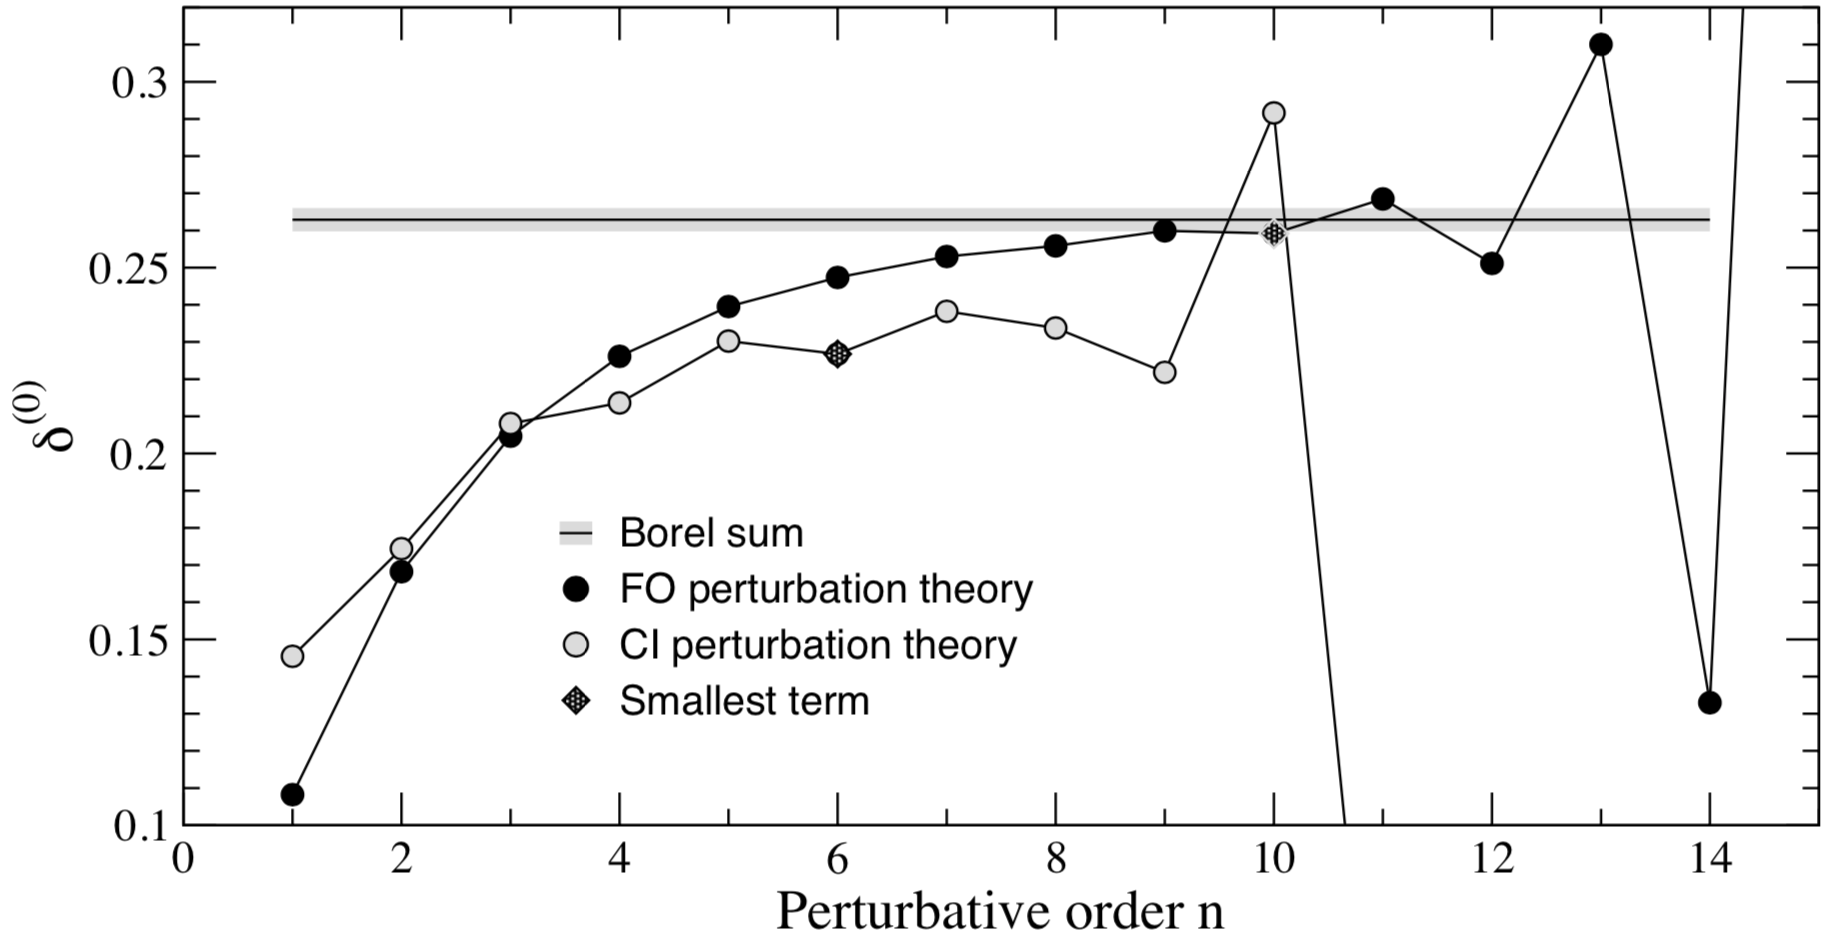
\includegraphics[width=0.7\textwidth]{./images/FOPT_CIPT_contributions.png}
    \end{center}
    \scriptsize \cite{Jamin2013a}
  \end{itemize}
\end{frame}
\note[itemize]{
\item FOPT and CIPT lead to different PT contributions
\item CIPT has smaller contributions \(\Rightarrow\) larger \(\alpha_s\)
\item Plot comparing FOPT, CIPT and BS from Beneke and Jamin
\item Black dots FOPT, gray dots CIPT, black line BS 
\item Beneke and Jamin introduced Borel model
\item FOPT converges on BS line, CIPT does not \(\Rightarrow\) FOPT more valid
\item Will follow this strategy within our fits
}

\begin{frame}
  \frametitle{Borel Summation}
  \begin{itemize}
  \item Borel summation is a summation method for divergent asymptotic series,
    e.g. Adler function
  \item Beneke and Jamin introduced a physical model of the Adler
    function\footcite{Beneke2008}:
    \begin{equation}
      \label{eq:borelModel}
      B[\widehat D](u) = B[\widehat D_1^{UV}](u) + B[\widehat D_2^{IR}](u) + B[\widehat D_3^{IR}](u) + d_0^{PO} + d_1^{PO}u,
    \end{equation}
  \item Using the Borel integral we can recover the Adler function
    \begin{equation}
      \widehat D(\alpha) \equiv \int_0^\infty \dif t e^{-t/\alpha} B[\widehat D](t)
    \end{equation}
  \end{itemize}
\end{frame}
\note[itemize]{
\item Summation method for divergent asymptotic series
\item Best possible sum for Adler function
\item Beneke and Jamin (2008) modelled the Adler function
\item Have given Borel transform of the model
\item Adler function from Borel integral
\item Will apply model in fits to make a statement in the FOPT vs CIPT discussion
}

\begin{frame}
  \frametitle{Non-Perturbative Contributions}
  \begin{itemize}
  \item Neglect dimension two contributions
  \item Dimension four vacuum condensate contributions:
    \begin{equation}
      D_{4} = \frac{1}{12}\left[ 1 - \frac{11}{18}a_s \right] \langle  a_s GG \rangle
      + \left[ 1 + \frac{\pm 36 - 23}{27} a_s \right] \langle (m_u + m_d) \overline{q}q \rangle
    \end{equation}
  \item We work with the invariant gluon condensate
    \begin{equation}
      \langle a_s GG \rangle_I \approx 0.021
    \end{equation}
  \item Higher dimensional contributions are approximated by simplest possible
    approach:
    \begin{small}
      \begin{equation}
        D_{6} = 3 \frac{\rho_{V/A}^{(6)}}{s^3}, \quad
        D_{8} = 4 \frac{\rho_{V/A}^{(8)}}{s^4}, \quad
        D_{10} = 5 \frac{\rho_{V/A}^{(10)}}{s^5}, \quad
        D_{12} = 6 \frac{\rho_{V/A}^{(12)}}{s^6}
      \end{equation}
    \end{small}
  \end{itemize}
\end{frame}
\note[itemize]{
\item Neglect dimension two contributions, because proportional to quark masses
\item The D=4 contributions can be expressed as: Gluon condensate and quark
  condensate with corresponding factor. Also depend on \(m^4\)
\item We use Invariant Gluon, we will fit the gluon condensate
\item D=6 and higher approximated by simplest approach possible: \(\rho\)
  constants divided by corresponding \(1/s\) term
\item Fit up to dimension 12
}

\subsection{Experimental Data}
\begin{frame}
  \centering \vspace{0.5cm}
  \begin{LARGE}
    The Experimental Data
  \end{LARGE}
  \begin{equation}
    I^{exp}(s_0) \equiv \frac{12 \pi^2}{s_0} \int_0^{s_0} \dif s \omega\left(\frac{s}{s_0}\right) \rho^{exp}_{V/A}(s)
  \end{equation}
\end{frame}

\begin{frame}
  \frametitle{Inclusive Hadronic Tau Decay Ratio}
  \begin{itemize}
  \item Spectral function \(\rho(s)\) is a measurable from the inclusive
    hadronic tau decay ratio
    \begin{equation}
      R_\tau = \frac{\Gamma[\tau^- \to \nu_\tau + \text{hadrons}]}{\Gamma[\tau^- \to \nu_\tau e^- \overline{\nu}_{e}]} = 3.6349(82)\footcite{HFLAV2016}
    \end{equation}
  \item We work with the inclusive non-strange tau decay ratio
    \begin{equation}
      R_{\tau, V+A} = R_\tau - R_{\tau,s} = 3.4718(72)^3
    \end{equation}
  \item Inclusive Hadronic Tau Decay Ratio is given by (\(s \equiv -q^2\))
    \begin{scriptsize}
      \begin{equation}
        R_{\tau, V+A} = 12 \pi \,\abs{V_{ud}}^2 S_{EW} \int_0^{m_\tau^2} \frac{\dif s}{m_\tau^2} \left( 1 + 2 \frac{s}{m_\tau^2} \right)
        \left[ \left( 1+2\frac{s}{m_\tau^2} \right) \Ima \Pi_{V+A}^{(1)}(s) + \Ima \Pi_{V+A}^{(0)}(s)\right]
      \end{equation}
    \end{scriptsize}
  \end{itemize}
\end{frame}
\note[itemize]{
\item A central value is the inclusive hadronic tau decay ratio (i.e. all decays
  containing hadrons)
\item The ratio can be calculated by using the optical theorem
\item \(V_{ud}\) is the Cabbibo matrix element, \(S_{EW}\) the electroweak
  correction
\item We have to integrate the two-point function from \(0 \to m_\tau^2\)
\item The two-point function has poles on the positive real axis, on the
  remaining \(s\) plane the two-point function is analytic
\item \(\Pi^{(0)}\) will be neglected? There is no \(J=0\) vector contribution.
  The \(J=0\) axial-vector contribution is the pion pole. Which is missing in
  the experimental data.
}

\begin{frame}
  \frametitle{ALEPH Data}
  \begin{itemize}
    \item V (left) and A (right) channel of the Aleph data
    \begin{columns}
      \begin{column}{0.5\textwidth}
        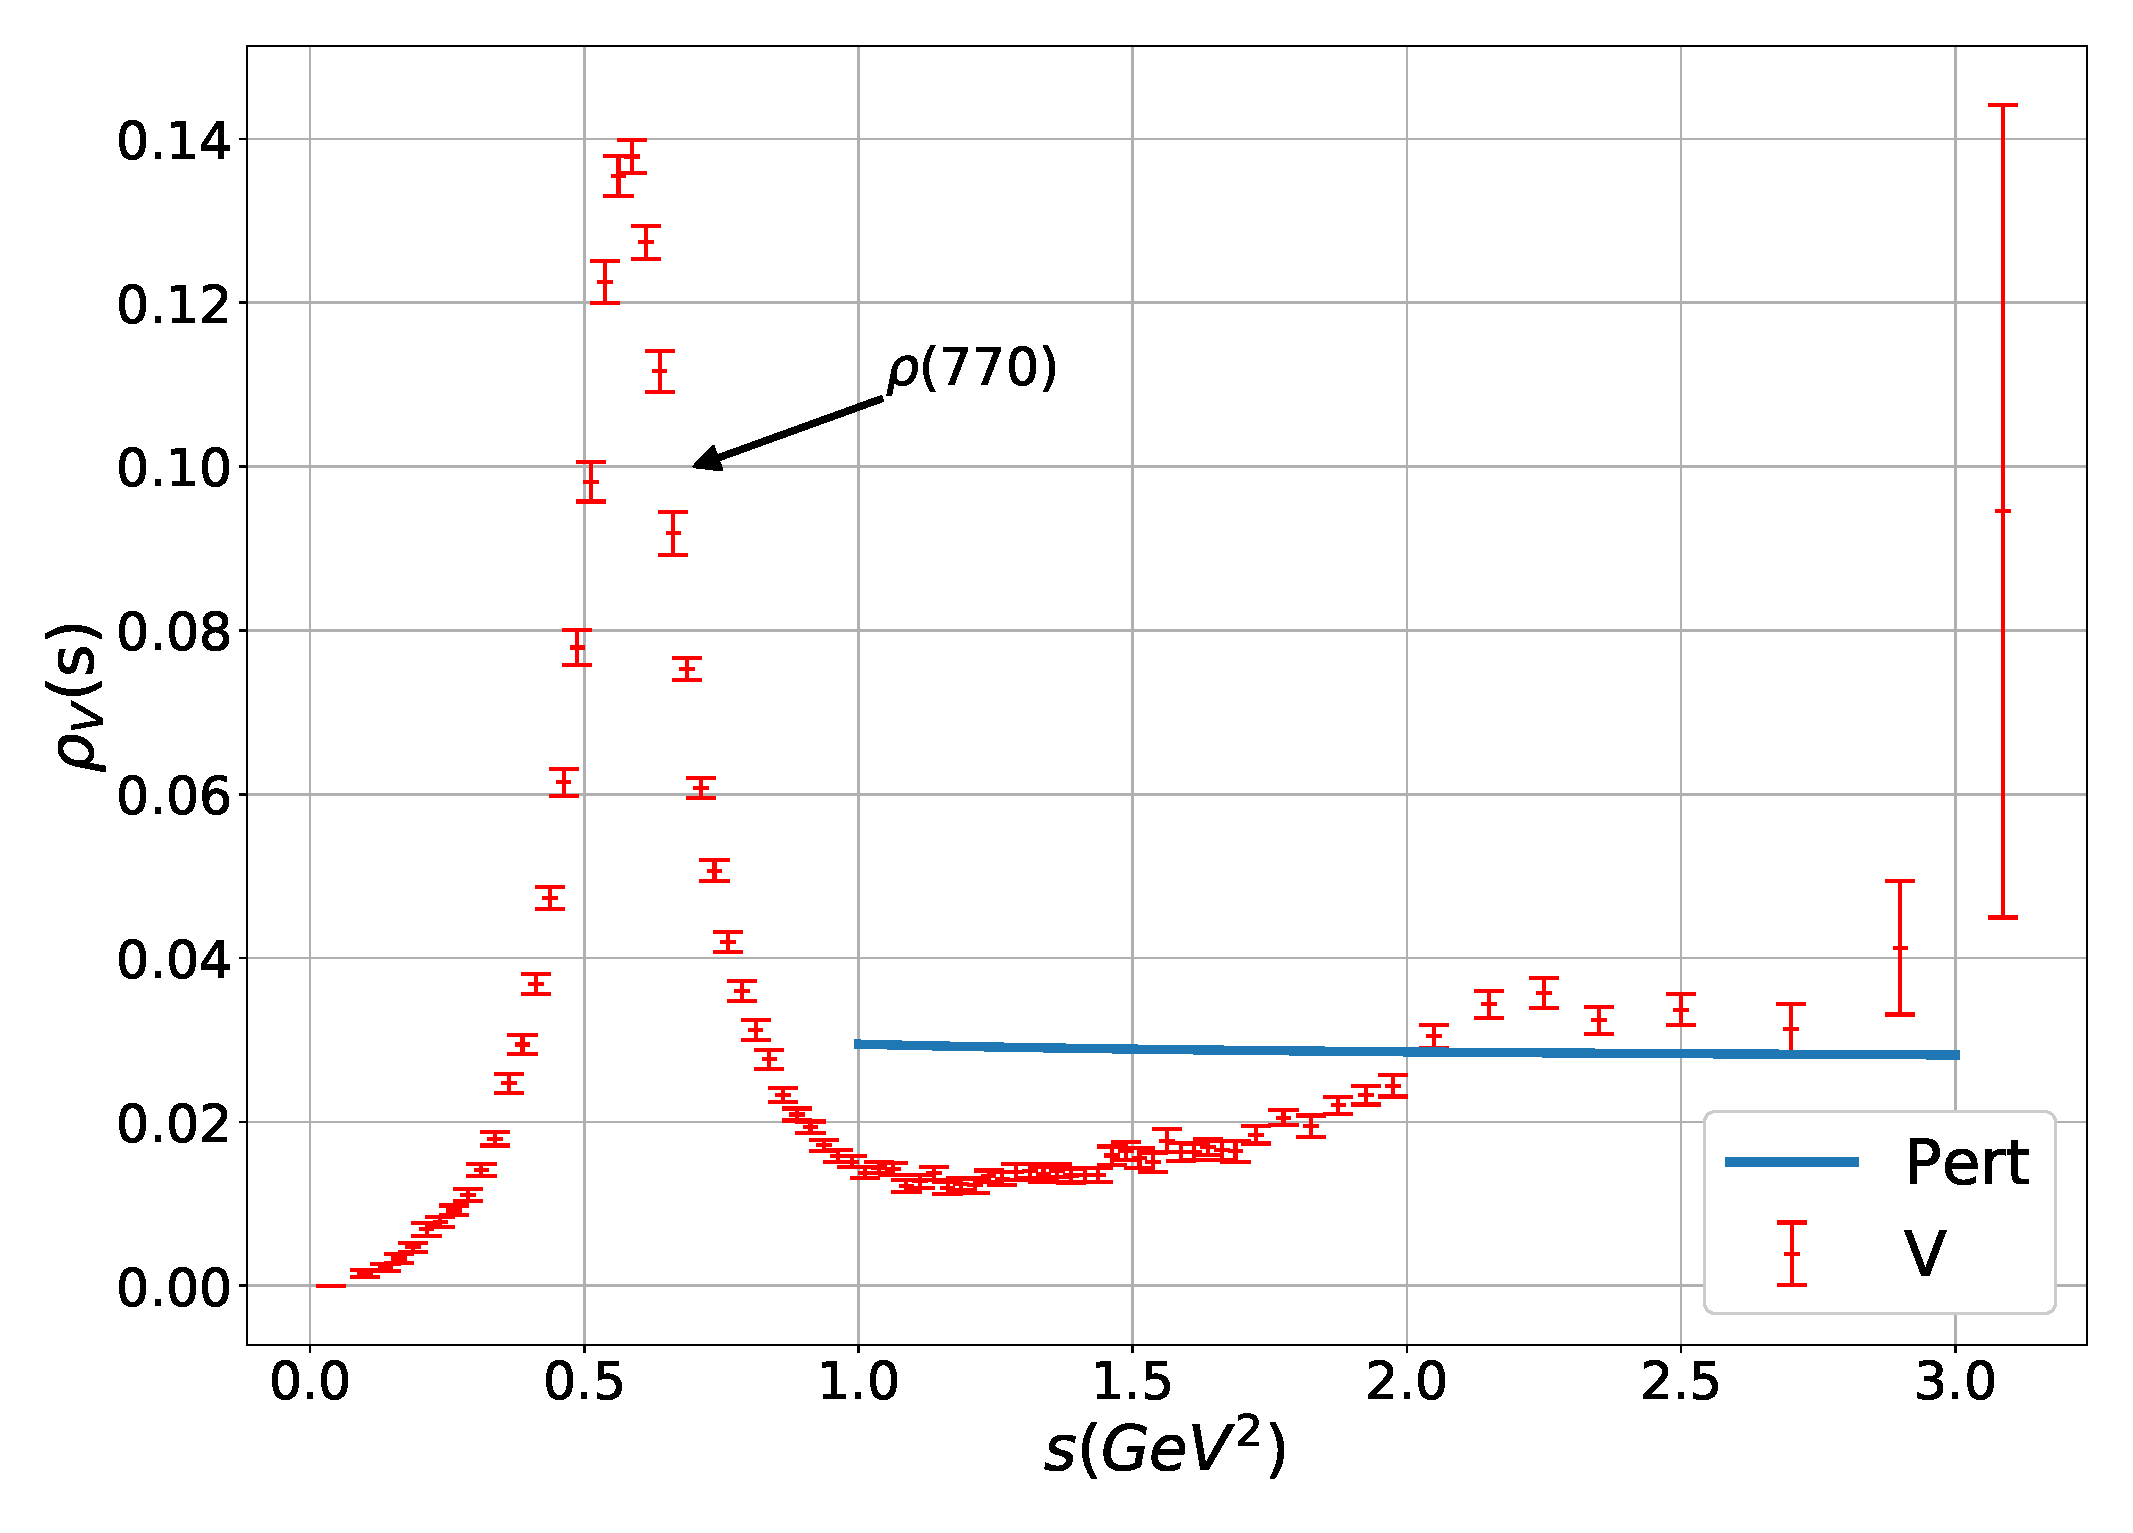
\includegraphics[width=\textwidth]{./images/specFuncAleph_V.eps}
      \end{column}
      \begin{column}{0.5\textwidth}
        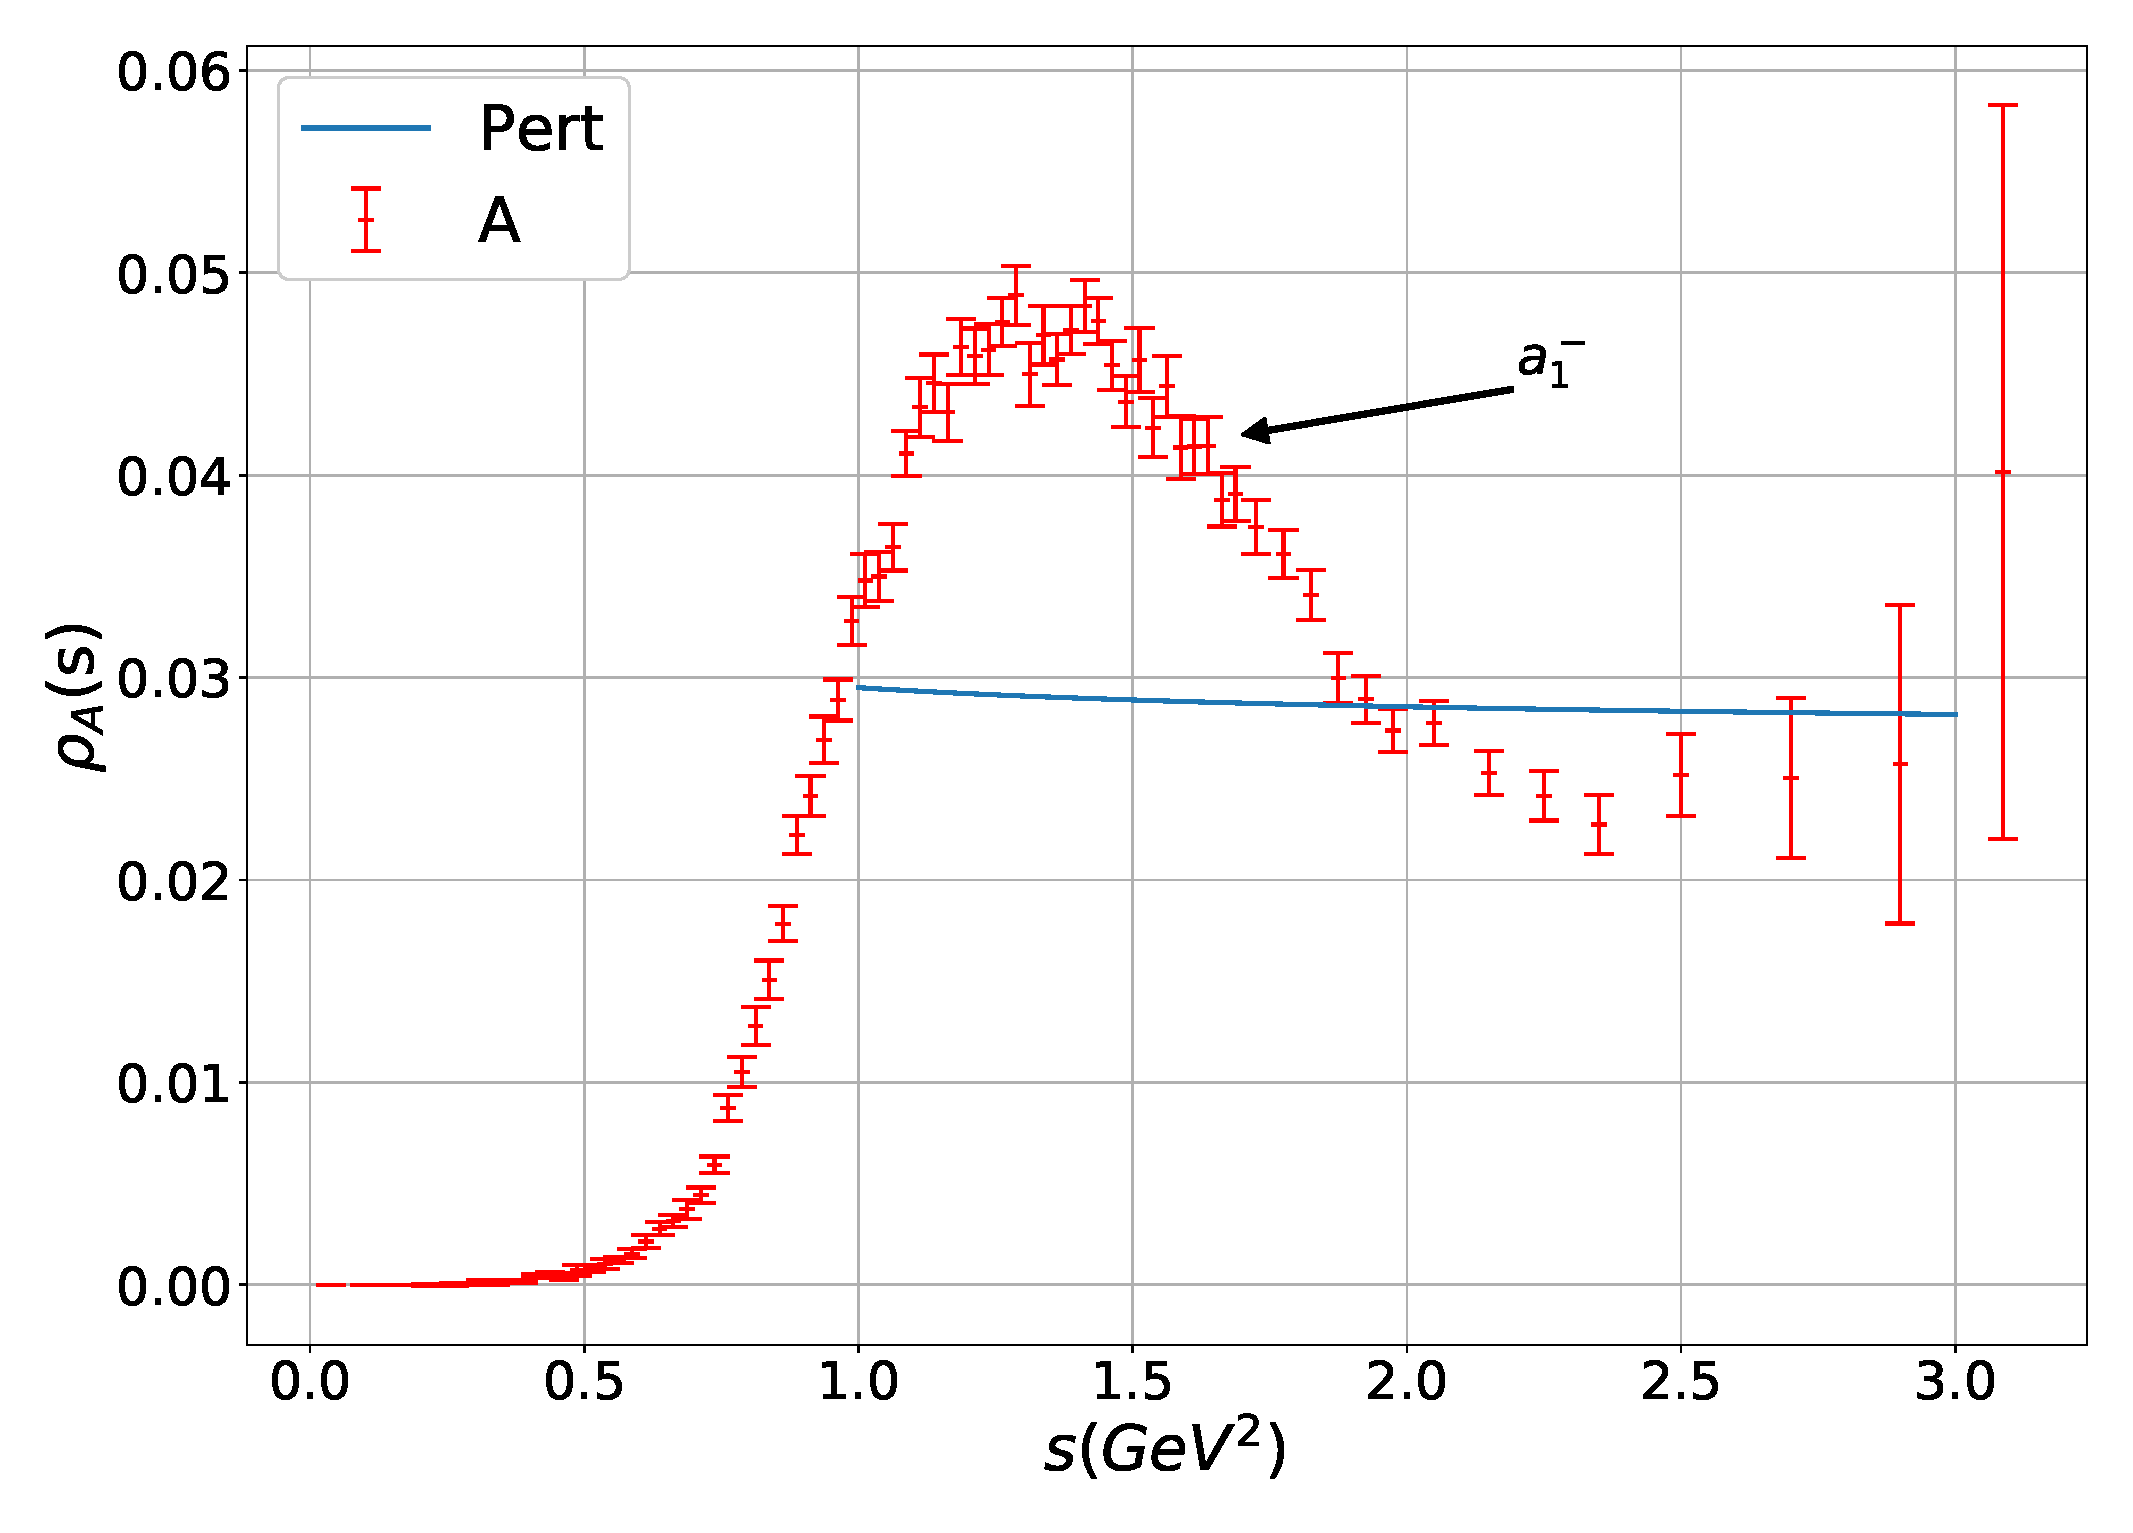
\includegraphics[width=\textwidth]{./images/specFuncAleph_A.eps}
      \end{column}
    \end{columns}
  \item OPE cannot reproduce the data (especially for lower energies)
  \item e.g. the V and A channel D=6 contributions cancel
  \end{itemize}
\end{frame}
\note[itemize]{
\item The data we use is given by the ALEPH group
\item ALEPH was a particle detector on the Large Electron-Positron collider in
  the nineties
\item The data is given as a the normalised invariant mass squared distribution
  \(\dif N/ N/ \dif s\) for each channel \(V\), \(A\) and \(V+A\)
\item In the two graphs we see the contribution of the \(V\) channel (left) and
  the \(A\) channel (right)
\item In the vector channel we see the \(\rho(770)\) resonance
\item In the axial channel we see the \(a_1^-\) resonance
\item We also plotted the Perturbative contribution, which cannot reproduce the
  experimental data, especially for lower energies
}

\begin{frame}
  \frametitle{ALEPH Data}
  \begin{itemize}
  \item ALEPH V+A channel
    \begin{center}
      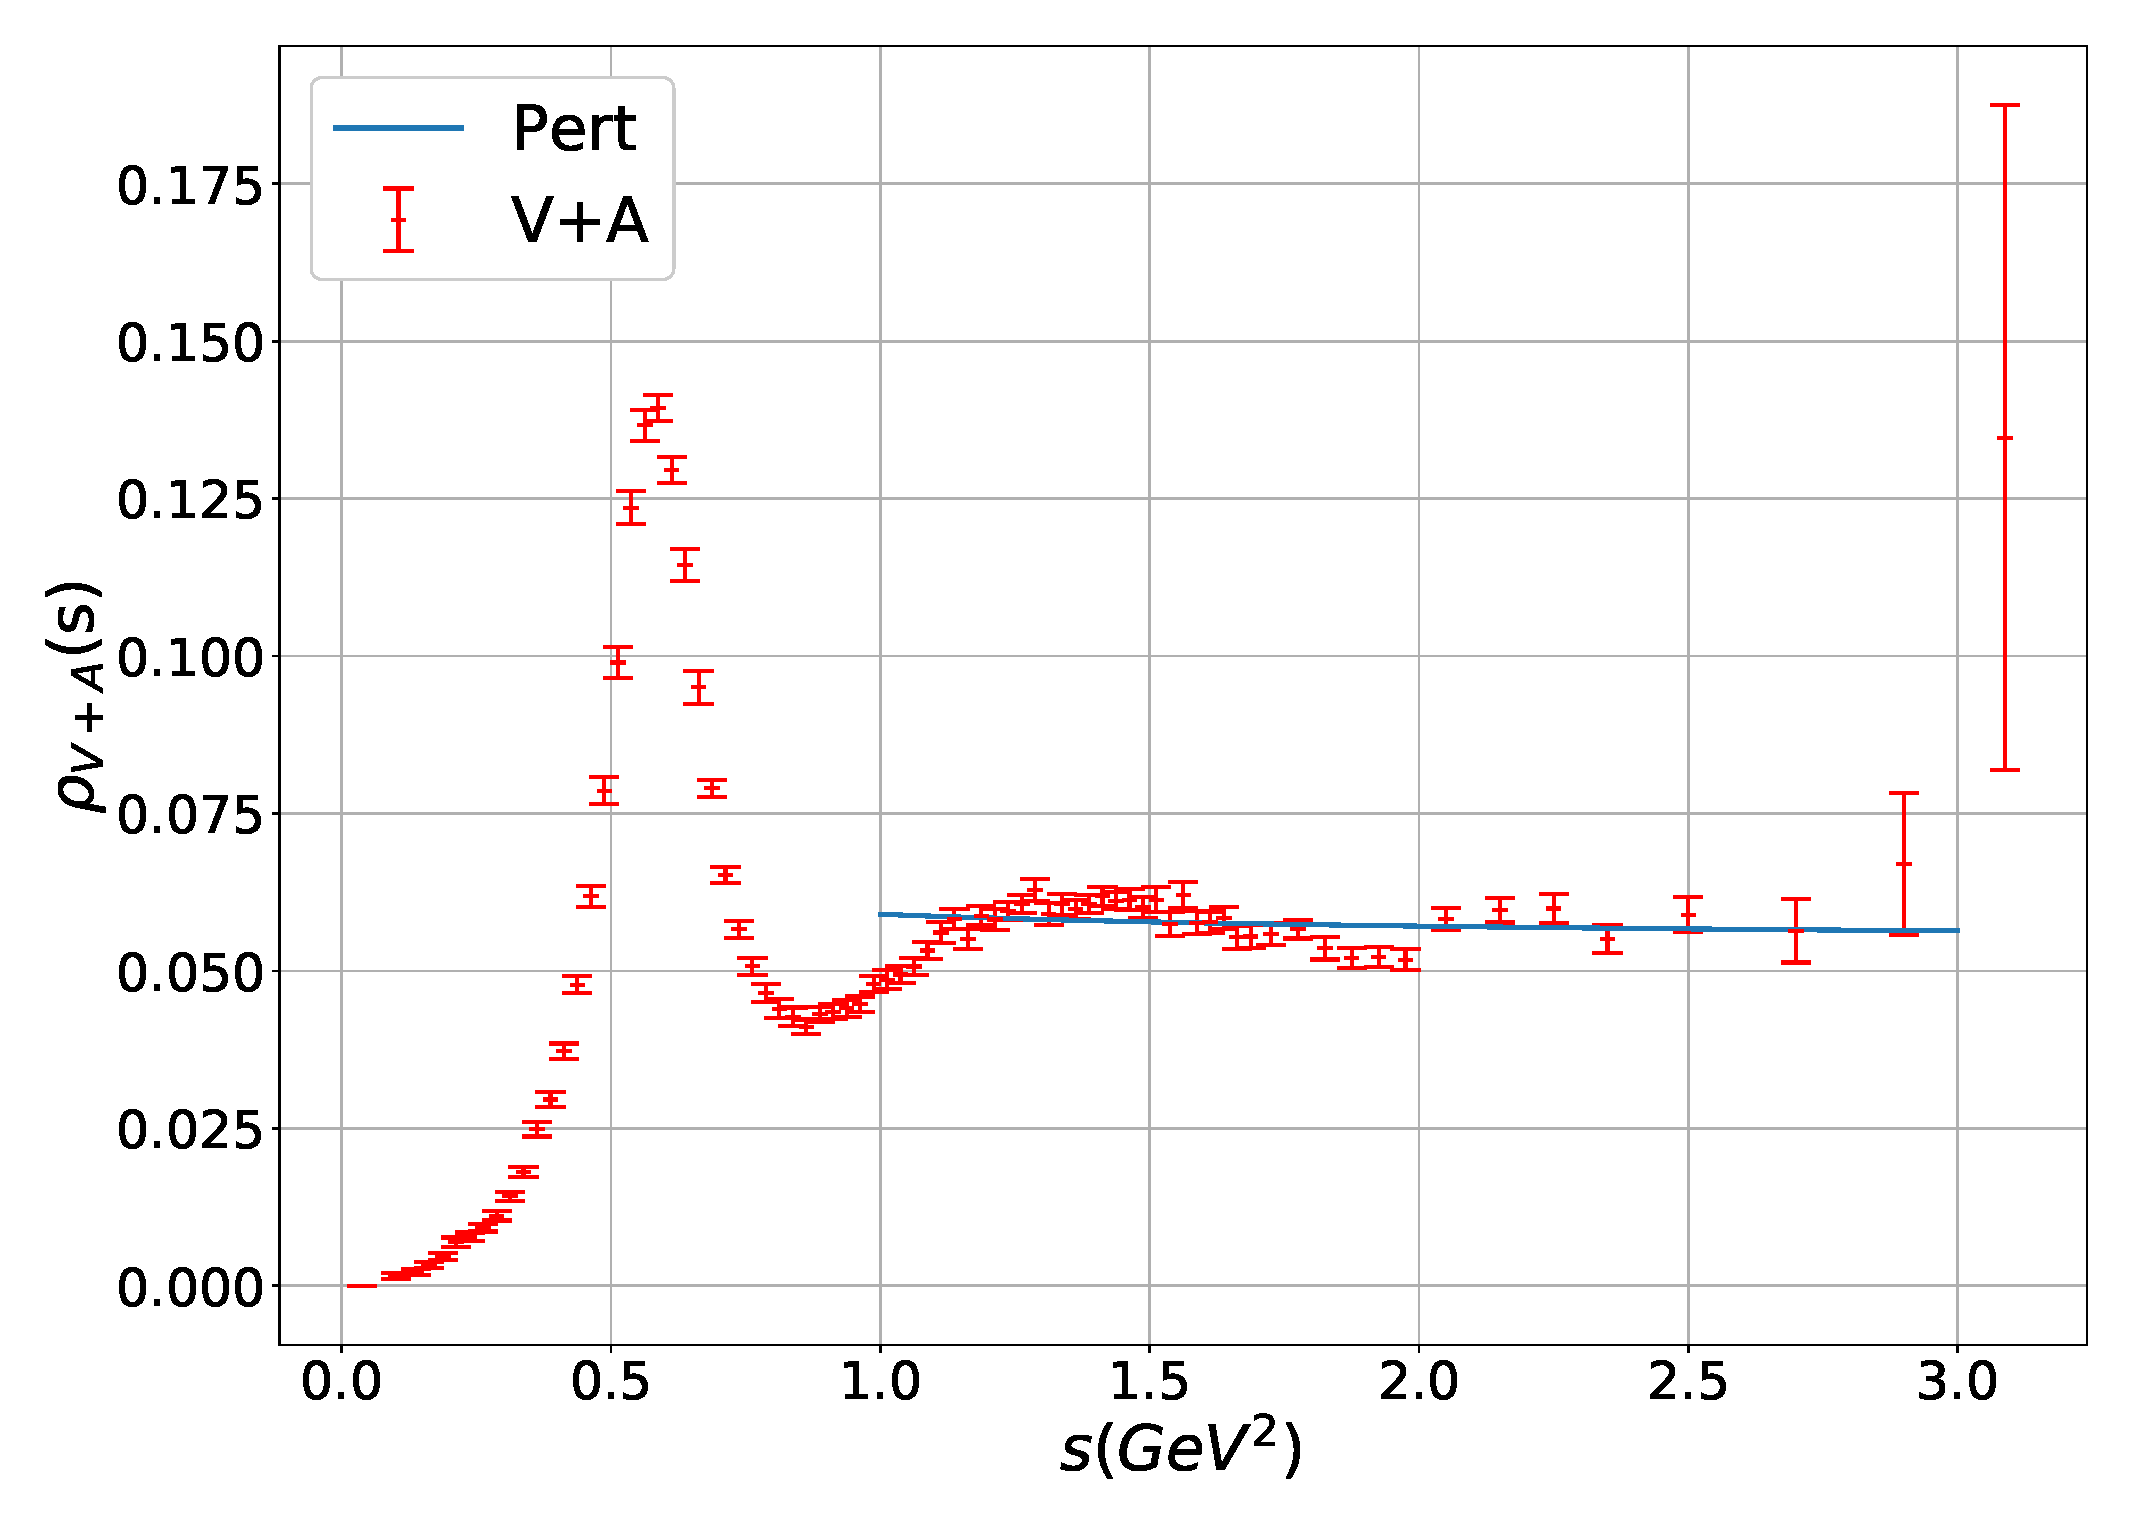
\includegraphics[width=.8\textwidth]{./images/specFuncAleph_VpA.eps}
    \end{center}
  \item The OPE is suppressed in the V+A channel
  \end{itemize}
\end{frame}
\note[itemize]{
\item OPE is suppressed in the V+A channel \(\Rightarrow\) NPT contributions smalDV also suppressed
\item Here we see the experimental spectral function of the \(V+A\) channel
\item Note that for higher energies the perturbative contribution matches the
  spectral function far better
\item Also note that we still see a wavy behaviour of the spectral function in
  the data, which is connected to Duality Violations
\item We assume that in the \(V+A\) channel DV are sufficiently suppressed to
  avoid modelling their contributions }

\begin{frame}
  \frametitle{Experimental Spectral Functions}
  \begin{itemize}
  \item Experimental Spectral Functions:
    \begin{align}
      \frac{1}{N} \frac{\Delta N_{V/A}^{(1)}(s_i)}{\Delta s_i}
      &\approx \frac{1}{N} \frac{\dif N_{V/A}^{(1)}}{\dif s} = B_e \frac{\dif R_{\tau, V/A}^{(1)}}{\dif s}(s) \nonumber\\
      &= \frac{12\pi^2}{m_\tau^2} B_e S_{EW} \abs{V_{ud}}^2
        \left( 1 - \frac{s}{m_\tau^2} \right)^2\left( 1 + \frac{2s}{m_\tau^2} \right) \rho_{V/A}^{(1)}(s) \\
      \frac{1}{N} \frac{\Delta N_{V/A}^{(0)}(s_i)}{\Delta s_i}
      &\approx \frac{1}{N} \frac{\dif N_{V/A}^{(0)}}{\dif s} = B_e \frac{\dif R_{\tau, V/A}^{(0)}}{\dif s}(s) \nonumber\\
      &= \frac{12\pi^2}{m_\tau^2} B_e S_{EW} \abs{V_{ud}}^2
        \left( 1 - \frac{s}{m_\tau^2} \right)^2 \rho_{V/A}^{(0)}(s)
    \end{align}
  \item \(\Delta N_{V/A}^{(0,1)}(s_i)\) is the number of \(V/A\) events with
    \(J=0,1\) in the bin centred at \(s_i\).
  \end{itemize}
\end{frame}


\section{Fits}
\subsection{Strategy}
\begin{frame}
  \frametitle{Chi-Squared}
  \begin{itemize}
    \item The integral moments depend on the weight \(\omega\) and selected
      energy \(s_0\)
      \begin{equation*}
        \begin{split}
          I^{th}(s_0, \omega) \quad \text{and} \quad I^{exp}(s_0, \omega)
        \end{split}
      \end{equation*}
    \item For a fit we choose a weight and select multiples \(s_0s\)
    \item The chi-squared is then given by:
      \begin{equation}
        \chi^2 = (I_i^{exp} - I_i^{th}(\vec \alpha)) C_{ij}^{-1} (I_j^{exp} - I_j^{th}(\vec \alpha)), \quad \text{with} \quad C_{ij} = \cov(I_i^{exp}, I_j^{exp})
      \end{equation}
    \item A typical fit then looks like this
      \begin{columns}
        \begin{column}{.4\textwidth}
          \begin{itemize}
          \item 9 Moments
          \item fit at most 8 parameters
          \end{itemize}
        \end{column}
        \begin{column}{.6\textwidth}
          \centering
          \begin{tabular}{cccc}
            \toprule
            \# &\multicolumn{3}{c}{9 Moments} \\
            \midrule
            1      & \(I_1\) & \(s_1\) & \(\omega\) \\
            2      & \(I_2\) & \(s_2\) & \(\omega\) \\
            \vdots & \cvdots & \vdots  & \vdots     \\
            9      & \(I_3\) & \(s_9\) & \(\omega\) \\
            \bottomrule
          \end{tabular}
        \end{column}
      \end{columns}
  \end{itemize}
\end{frame}
\note[itemize]{
  \item The chi-squared function is constructed from the theoretical and
    experimental moments
  \item The indices \(i\) and \(j\) represent the dependency of the moments on
    the chosen weight and \(s_0\)
  \item The fits are highly correlated.
  \item The correlation matrix is given with the data.
  \item A good fit is characterised by a \(\chi^2/dof \approx 1\) 
  \item As we have to deal with missing correlations, we will also interpret
    fits with a \(\chi^2/dof\) smaller than 1 as good
}

\begin{frame}
  \frametitle{How to choose Weights}
  \begin{itemize}
    \item Weight functions have to be analytic:
      \begin{equation}
        \omega(x) \equiv \sum_i a_i x^i
      \end{equation}
    \item We choose weights to two major criteria: pinching and contained monomials
    \item E.g. the kinematic weight
          \begin{equation}
            \begin{split}
              \omega_\tau &\equiv (1 - x)^2(1 + 2x) \\
              &= 1 - 3x^2 + 2x^3
            \end{split}
          \end{equation}
          \(\Rightarrow\) double pinched, no monomial term \(x\), D6 and D8
  \end{itemize}
\end{frame}
\note[itemize]{
  \item The weight is an analytic function
  \item Thus we can define it as an arbitrary polynomial
  \item As an example we can take the natural appearing kinetic weight \(\omega_\tau\)
  \item It is double pinched, does not contain a monomial and as we will see has
    active D6 and D8 contributions
  \item next slide shows pinching and active OPE contributions
}

\begin{frame}
  \frametitle{How to choose Weights}
  \begin{itemize}
  \item Pinched weight suppress the correlator close to the not analytic
    positive real axis, which is known for Duality Violations
    \begin{equation}
      \omega(x) = \left( 1 - x \right)^k
    \end{equation}

    \vfill

    \item The active OPE Dimensions depend on the monomials the weight carries:
      \begin{equation}
        \oint_{C} x^k \dif x = i \int_0^{2\pi}\left(e^{i \theta}\right)^{k+1} \dif \theta
        = \begin{cases} \mbox{\(2 \pi i\)} & \mbox{if } k=-1, \\ \mbox{0} & \mbox{otherwise} \end{cases}.
      \end{equation}
      \begin{equation}
        R(x)\biggr\rvert_{D=0,2,4,\dots} = \oint_{\abs{x}=1} \dif x \, x^{k-D/2} C^{(D)} \quad \Rightarrow \quad D = 2 (k+1)
      \end{equation}
      \begin{tabular}{l|cccccc}
        \toprule
        \textbf{monomial:} & \(x^0\) & \(x^1\) & \(x^2\) & \(x^3\) & \(x^5\) & \(x^6\)\\
        \textbf{dimension:} & \(D^{(2)}\) & \(D^{(4)}\) & \(D^{(6)}\) & \(D^{(8)}\) & \(D^{(10)}\) & \(D^{(12)}\)\\
        \bottomrule 
      \end{tabular}
  \end{itemize}
\end{frame}
\note[itemize]{
  \item The theoretical two-point function contains DV close to the positive
    real axis
  \item To suppress DV contributions we introduce pinched weights
  \item The order of the pinching is given by the exponent \(k\) in equation 50
  \item The higher the pinching the fewer the contributions close to the
    positive real axis. This can be seen by plotting the weights. Blue is single
    pinched and decreases linear. Higher pinched weights decrease faster.
  \item Thus implementing a sufficient pinching should avoid DV
  \item PT contributes due to logarithms
  \item Also other dimensions can contribute due to logarithmic energy dependecies
  \item Took OPE contributions as constant, in reality have logarithmic
    dependencies so actually contribute
  \item Always include D4 due to logarithmic contributions
  \item Logs are in Wilson coefficients
}

\begin{frame}
  \frametitle{Strategy}
  \begin{itemize}
    \item Extract \(\alpha_s\)
    \item Probe Duality Violations
      \begin{itemize}
        \item Fit different pinched weights
        \item If similar values \(\Rightarrow\) DV sufficiently suppressed
      \end{itemize}
    \item FOPT vs CIPT
      \begin{itemize}
        \item Fits using FOPT and BS
        \item If similar values \(\Rightarrow\) FOPT more value
      \end{itemize}
    \end{itemize}
\end{frame}
\note[itemize]{
  \item To extract \(\alpha_s\) at the \(m_\tau^2\) scale, we perform fits with
    multiple \(s_0\) moments.
  \item We check isolated weights for stability for different \(s_0\) moments
  \item Check stability for different weights and pinchings. If we obtain
    similar weights DV should not be present.
  \item Perform additional fits with the BS. If parameters are similar to FOPT,
    then FOPT should be the preferred framework.
}

\begin{frame}
  \frametitle{Chosen Weights}
  \resizebox{\textwidth}{!}{
    \begin{tabular}{ccccc}
      \toprule
      & Symbol & Term & Expansion & \textsc{ope} Contributions \\
      \midrule
      \parbox[t]{2mm}{\multirow{3}{*}{\rotatebox[origin=c]{90}{\small Pinched}}} & \(\omega_\tau\) & \((1-x)^2(1+2x)\) & \(1 - 3x^2 + 2x^3\) & \(D6, D8\) \\
      & \(\omega_{cube}\) & \((1-x)^3(1+3x)\) & \(1 - 6x^2 + 8x^3 - 3x^4\) & \(D6, D8, D10\) \\
      & \(\omega_{quartic}\) & \((1-x)^4(1+4x)\) & \(1 - 10x^2 + 20x^3 - 15x^4 + 4x^5\) & \(D6, D8, D10, D12\) \\
      \midrule
      \parbox[t]{2mm}{\multirow{3}{*}{\rotatebox[origin=c]{90}{\small Monomial}}} & \(\omega_{M2}\) & \(1 - x^2\) & \(1-x^2\) & \(D6\) \\
      & \(\omega_{M3}\) & \(1 - x^3\) & \(1 - x^3\) & \(D8\) \\
      & \(\omega_{M4}\) & \(1 - x^4\) & \(1 - x^4\) & \(D10\) \\
      \midrule
      \parbox[t]{2mm}{\multirow{4}{*}{\rotatebox[origin=c]{90}{\small Pinched \(+ x\)}}} & \(\omega_{1,0}\) & \((1 - x)\) & \(1 - x\) & \(D4\) \\
      & \(\omega_{2,0}\) & \((1 - x)^2\) & \(1 - 2x + x^2\) & \(D4, D6\) \\
      & \(\omega_{3,0}\) & \((1 - x)^3\) & \(1 - 3x + 3x^2 - x^3\) & \(D4, D6, D8\) \\
      & \(\omega_{4,0}\) & \((1 - x)^4\) & \(1 - 4x + 6x^2 - 4x^3 + x^4\) & \(D4, D6, D8, D10\) \\
      \bottomrule
    \end{tabular}
  }
\end{frame}
\note[itemize]{
  \item To apply the strategy we have to choose several weights
  \item We selected three categories:
    \begin{itemize}
      \item Pinched weights without a monomial term
        \(x\), these are double, triple or quadruple pinched,  
      \item Monomial weights, these weights are single pinched and do not
        contain a monomial term \(x\)
      \item ``Pichs optimal'' weights, these weights are single up to quadruple
        pinched and contain a term monomial in \(x\)
    \end{itemize}
  \item We cannot apply FOPT to weights with a monomial term \(x\)
    \(\Rightarrow\) BS
  \item studied quadruple pinched weights but exclude from results, converge
    bad, but their results are in line with our other weights
}

\subsection{Results}
\begin{frame}
  \frametitle{Kinematic Weight: \(\omega_\tau(x) \equiv (1-x)^2(1+2x)\)}
  \centering
  \begin{tabular}{ccccccc}
    \toprule
    & \(s_{min} [GeV^2]\) & \#\(s_0\)s & \(\alpha_s(m_\tau^2)\) & \(\rho^{(6)}\) & \(\rho^{(8)}\) & \(\chi^2/dof\)  \\
    \midrule
    \parbox[t]{2mm}{\multirow{5}{*}{\rotatebox[origin=c]{90}{\textsc{fopt}}}}
    % 1.500 & 23 & 0.3255(13) & -0.441(10) & -0.2909(34) & 2.00 \\
    % 1.525 & 22 & 0.3255(18) & -0.440(36) & -0.288(45) & 2.10 \\
    % 1.550 & 21 & 0.3265(16) & -0.478(36) & -0.343(50) & 1.81 \\
    % 1.575 & 20 & 0.3269(22) & -0.493(47) & -0.365(58) & 1.86 \\
    % 1.600 & 19 & 0.3272(23) & -0.506(51) & -0.384(64) & 1.94 \\
    % 1.625 & 18 & 0.3284(24) & -0.540(53) & -0.433(68) & 1.788 \\
    % 1.650 & 17 & 0.3283(24) & -0.550(57) & -0.448(74) & 1.90 \\
    % 1.675 & 16 & 0.3284(24) & -0.549(57) & -0.448(79) & 2.04 \\
    % 1.700 & 15 & 0.3281(24) & -0.538(63) & -0.430(87) & 2.19 \\
    % 1.750 & 14 & 0.3291(26) & -0.581(71) & -0.50(10) & 2.21 \\
    % 1.800 & 13 & 0.3293(27) & -0.589(77) & -0.51(11) & 2.43 \\
    % 1.850 & 12 & 0.3281(28) & -0.537(85) & -0.42(13) & 2.5 \\
    % 1.900 & 11 & 0.3272(29) & -0.493(93) & -0.35(15) & 2.65 \\
    % 1.950 & 10 & 0.3232(32) & -0.31(11) & -0.01(18) & 1.13 \\
    % 2.000 & 9 & 0.3234(34) & -0.32(12) & -0.03(21) & 1.31 \\
    & \(2.1\) & 8 & 0.3256(38) & -0.43(15) & -0.25(28) & 1.30 \\
    & \cellcolor{primary}\(2.2\) & \cellcolor{primary}7 & \cellcolor{primary}0.3308(44) & \cellcolor{primary}-0.72(20) & \cellcolor{primary}-0.85(38) & \cellcolor{primary}0.19 \\
    & \(2.3\) & 6 & 0.3304(52) & -0.69(25) & -0.80(50) & 0.25 \\
    & \(2.4\) & 5 & 0.3339(70) & -0.91(39) & -1.29(83) & 0.10 \\
    & \(2.6\) & 4 & 0.340(15) & -1.3(1.0) & -2.3(2.5) & 0.01  \\
    \midrule
    \parbox[t]{2mm}{\multirow{1}{*}{\rotatebox[origin=c]{90}{\textsc{bs}}}}
    & \(2.2\) & 7 & 0.3274(42) & -0.82(21) & -1.08(41) & 0.21 \\
    \bottomrule
  \end{tabular}
\end{frame}
\note[itemize]{
  \item Kinematic weight is double pinched (suppressed DV), contains no monomial term x
  \item OPE D=6 and D=8
  \item Three fitting parameters: \(\alpha_s, \rho^{(6)}\) and \(\rho^{(8)}\)
  \item \(s_{min}\) smallest invariant mass squared value
  \item Probed weight down to \SI{1.5}{\giga\eV}
  \item Increasing number of \(s_0\)'s the \(\chi^2/dof\) increases, until point
    where \(\chi^2/dof\) jumps (threshold/ phase transition)
  \item \(s_0\) becomes to low for a good theoretical description
  \item Select fits with maximum number of \(s_0\) that is still below above
    \(s_0\) threshold as best fit (blue background)
  \item Same behaviour in all fits, also select best fit
  \item Parameters are within the weight very stable \(\alpha_s \approx 0.33\)
  \item We are aware that the \(\chi^2/dof\) are small, caused by missing correlations
  \item Performed BS for best fit, also compatible
  \item CIPT causes higher values for \(\alpha_s\) \(\Rightarrow\) FOPT more valid
}

\begin{frame}
  \frametitle{Comparison}
  \centering \resizebox{\textwidth}{!}{
    \begin{tabular}{cccccccc}
      \toprule
      weight & PT & \(\#s_0\)'s & \(\alpha_s(m_\tau^2)\) & \(10^2\langle aGG \rangle_I\) & \(10^2\rho^{(6)}\) & \(10^2\rho^{(8)}\) & \(\chi^2/dof\)  \\
      \midrule
      \((1-x)^2(1 + 2x)\)    & FO & 7 & 0.3308(44) & \(2.1^*\) & -0.72(20) & -0.85(38) & 0.19 \\
      \((1-x)^2(1 + 2x)\)  & BS & 7 & 0.3274(42) & \(2.1^*\)    & -0.82(21)   & -1.08(41) & 0.21 \\
      \((1-x)^3(1+2x)\)    & FO & 8 & 0.3302(40) & \(2.1^*\) & -0.52(11) & -0.58(22) & 0.43 \\ 
      % & \(\omega_{quartic}\) & 2.0 & 0.3290(11) & - & -0.3030(46) &
      % -0.1874(28) & 0.3678(45) & 0.67 \\
      \(1 - x^2\)          & FO & 7 & 0.3248(52) & \(2.1^*\) & -0.77(22) & \(0^*\)   & 0.38 \\
      \(1 - x^3\)          & FO & 7 & 0.3214(49) & \(2.1^*\) & \(0^*\)   & -1.01(39) & 0.41 \\
      % & \(\omega_{M4}\) & 2.2 & 0.3203(48) & - & - & - & -1.64(77) & 0.42 \\
      \(1 - x\)           & BS & 7 & 0.3246(52) & -2.26(59)  & \(0^*\)     & \(0^*\)   & 0.38 \\
      \(1 - x\)           & FO & 7 & 0.352(15)  & -6.54(29)  & \(0^*\)     & \(0^*\)   & 0.27 \\
      \((1 - x)^2\)       & BS & 7 & 0.3270(54) & -2.54(61)  & -0.77(21)   & \(0^*\)   & 0.74 \\
      \((1 - x)^2\)       & FO & 7 & 0.3401(58) & -1.86(53)  & 0.22(9)     & \(0^*\)   & 0.73 \\
      \((1 - x)^3\)       & BS & 8 & 0.3239(51) & -2.12(55)  & -0.63(19)   & -0.74(36) & 0.46 \\
      % & \(\omega_X4}\) & 2.1 & 0.3248(21) & -0.02230(47) & -0.6724(63) &
      % -0.834(14) & -1.352(28) & 0.23 \\
      \bottomrule
    \end{tabular}
    }
\end{frame}
\note[itemize]{
  \item Gathered the ``best'' fits (from phase transition)
  \item Fits of different pinching
  \item We left out the fourth pinched weights (fits did not converge)
  \item Parameters with asterisks have been fixed
  \item Weights higher dimensional OPE omitted
  \item \(\alpha_s\) compatible
  \item \(\rho^{(6)}\), \(\rho^{(8)}\)  within error boundaries
  \item \(\Rightarrow\) DV are sufficiently suppressed
  \item Applied BS to weights containing \(x\)
  \item Still stable \(\Rightarrow\) FOPT valid
  \item BS yields \(\langle a GG \rangle\) with opposite sign, has to be investigated
}


\section{Conclusions}
\begin{frame}
  \frametitle{Conclusions}
  \begin{itemize}
  \item Obtained values for the strong coupling:
    \begin{equation*}
      \begin{split}
        \alpha_s(m_\tau^2) &= 0.3268(44)(25) = 0.3268(51) \\
        % \alpha_s^{(FOPT+BS)}(m_\tau) &= 0.3263(44)(25) = 0.3263(51)
      \end{split}
    \end{equation*}
    \begin{small}First error taken from kinematic weight, second error \(c_{5,1} \pm 100\%\)\end{small}
    \begin{equation*}
      \begin{split}
        \alpha_s(m_Z^2) &= 0.11886(53)(30)(5) = 0.11886(61) \\
        % \alpha_s^{(FOPT+BS)}(m_Z) &= 0.11880(53)(30)(5) = 0.11880(61)
      \end{split}
    \end{equation*}
    \begin{small}Evolved using RunDec3, third error from using 5-loop or 4-loop evolution\end{small}
    \begin{equation*}
      \alpha_s^{(FLAG)} = 0.11823(81)\footcite{FLAG2019}
    \end{equation*}
  \item \(\rho^{(6)} = -0.68(20) \quad \text{and} \quad \rho^{(8)} = -0.80(38)\)
  \item DV sufficiently suppressed (V+A channel and single pinched weights)
  \item FOPT more valid than CIPT
  \end{itemize}
\end{frame}


\begin{frame}
  \centering

  \vspace{0.5cm}

  \LARGE Questions
\end{frame}

\appendix
\begin{frame}
  \frametitle{Constants}
  \centering
  \begin{tabular}{lll}
    \toprule
    Quantity & Value \\
    \midrule
    \(V_{ud}\) & \(0.9742 \pm 0.00021\) \\
    \(S_{EW}\) & \(1.0198 \pm 0.0006\)  \\
    \(B_e\) & \(17.818 \pm 0.023\)      \\
    \(m_\tau\) & \SI{1.77686 \pm 0.12}{\mega\eV} \\
    \(\langle  a GG \rangle_I\) & \SI{0.012}{\giga\eV^2} \\
    \(\langle \anti{q}_{u/d}q_{u/d} \rangle(m_\tau) \) & \SI{-272 \pm 15}{\mega\eV} \\
    \( \anti{s}s / \langle \anti{q}q \rangle \) & 0.8 \pm 0.3 \\
    \bottomrule
  \end{tabular}
\end{frame}
\begin{frame}
  \frametitle{DV-model}
  \begin{equation}
    -\frac{1}{2 \pi i} \oint_{\abs{s}=s_0} \frac{\dif s}{s_0} \omega(s/s_0)
    \Delta_{V/A}(s) = - \int_{s_0}^\infty \frac{\dif s}{s_0} \omega(s/ s_0) \frac{1}{\pi} \Ima \Delta_{V/A}(s)
  \end{equation}
\end{frame}
\begin{frame}
  \frametitle{Pion Pole}
  \begin{ceqn}
    \begin{equation}
      R_{\tau,A}^\omega(s_0, \pi) = 24 \pi^2 \abs{V_{ud}}^2 S_{EW} \frac{f_\pi^2}{s_0}
      \omega \left( \frac{s_\pi}{s_0} \right)
      \left[ 1 - \frac{2 s_\pi}{s_\tau+ 2 s_\pi} \right]
    \end{equation}
  \end{ceqn}
\end{frame}
\begin{frame}
  \frametitle{Cubic Weight: \(\omega_{cube}(x) \equiv (1-x)^3(1+3x)\)}
  \begin{tabular}{ccccccc}
    \toprule
    \(s_{min}\) & \#\(s_0\)s & \(\alpha_s(m_\tau^2)\) & \(\rho^{(6)}\) & \(\rho^{(8)}\) & \(\rho^{(10)}\) & \(\chi^2/dof\)  \\
    \midrule
    % 1.800 & 13 & 0.3305(37) & -0.493(76) & -0.48(12) & -0.66(20) & 2.99 \\
    % 1.850 & 12 & 0.3303(37) & -0.482(68) & -0.456(100) & -0.62(17) & 3.35 \\
    % 1.900 & 11 & 0.3249(29) & -0.280(20) & -0.088(21) & 0.088(55) & 1.58 \\
    % 1.950 & 10 & 0.3237(26) & -0.232(25) & 0.005(42) & 0.275(93) & 1.67 \\
    2.000 & 9 & 0.3228(26) & -0.196(27) & 0.075(28) & 0.420(56) & 1.96 \\
    \rowcolor{primary}
    2.100 & 8 & 0.3302(40) & -0.52(11) & -0.58(22) & -1.00(45) & 0.43 \\
    2.200 & 7 & 0.3312(43) & -0.56(12) & -0.68(23) & -1.23(50) & 0.55 \\
    2.300 & 6 & 0.336(11) & -0.78(47) & -1.17(98) & -2.38(22) & 0.29 \\
    2.400 & 5 & 0.3330(96) & -0.63(47) & -0.82(10) & -1.51(26) & 0.48 \\
    \bottomrule
  \end{tabular}
\end{frame}
\note[itemize]{
  \item The cubic weight is triple pinched
  \item Has three active OPE contributions, \(D6, D8\), and \(D10\)
  \item Consequently we fitted four paremters
  \item Shows very similar behaviour to the kinematice weight (threshold, low
    \(\chi^2/dof\))
  \item Has also very stable values for \(\alpha_s\)
}

\begin{frame}
  \frametitle{Quartic Weight:  \( \omega_{quartic}(x) \equiv (1-x)^4(1+4x)\)}
  \begin{small}
    \begin{ceqn}
      \begin{equation}
        \begin{split}
          \alpha_s(m_\tau^2) = 0.3290(11), \quad \rho^{(6)}=-0.3030(46), \quad \rho^{(8)}=-0.1874(28), \\
          \rho^{(10)} = 0.3678(45) \quad \text{and} \quad \rho_{(12)}=-0.4071(77).
        \end{split}
      \end{equation}
    \end{ceqn}
  \end{small}
\end{frame}
\note[itemize]{
  \item Too many parameters. Only one fit converged
}
\subsubsection{Single Pinched Monomial Weights}
\begin{frame}
  \frametitle{\(\omega_{M2}(x) \equiv 1-x^2\)}
  \centering
  \begin{tabular}{ccccc}
    \toprule
    \(s_{min}\) & \#\(s_0\)s & \(\alpha_s(m_\tau^2)\) & \(\rho^{(6)}\) &  \(\chi^2/dof\)  \\
    \midrule
    2.100 & 8 & 0.3179(47) & -0.42(17) & 1.62 \\
    \rowcolor{primary}
    2.200 & 7 & 0.3248(52) & -0.77(22) & 0.38 \\
    2.300 & 6 & 0.3260(60) & -0.85(28) & 0.43 \\
    \bottomrule
  \end{tabular}
\end{frame}
\begin{frame}
  \frametitle{\(\omega_{M3}(x) \equiv 1-x^3\)}
  \centering
  \begin{tabular}{ccccc}
    \toprule
    \(s_{min}\) & \#\(s_0\)s & \(\alpha_s(m_\tau^2)\) & \(\rho^{(8)}\) &  \(\chi^2/dof\)  \\
    \midrule
    % 1.500 & 23 & 0.3160(28) & -0.523(65) & 2.4 \\
    % 1.525 & 22 & 0.3171(28) & -0.578(70) & 2.3 \\
    % 1.550 & 21 & 0.3173(29) & -0.587(76) & 2.42 \\
    % 1.575 & 20 & 0.3187(29) & -0.667(82) & 2.08 \\
    % 1.600 & 19 & 0.3189(30) & -0.679(87) & 2.19 \\
    % 1.625 & 18 & 0.3195(30) & -0.719(94) & 2.24 \\
    % 1.650 & 17 & 0.3205(30) & -0.783(99) & 2.1 \\
    % 1.675 & 16 & 0.3204(31) & -0.77(11) & 2.24 \\
    % 1.700 & 15 & 0.3206(31) & -0.79(11) & 2.39 \\
    % 1.750 & 14 & 0.3202(32) & -0.76(13) & 2.57 \\
    % 1.800 & 13 & 0.3217(33) & -0.88(14) & 2.41 \\
    % 1.850 & 12 & 0.3202(35) & -0.75(16) & 2.4 \\
    % 1.900 & 11 & 0.3202(36) & -0.75(18) & 2.67 \\
    % 1.950 & 10 & 0.3161(38) & -0.40(20) & 1.46 \\
    % 2.000 & 9 & 0.3148(39) & -0.28(22) & 1.47 \\
    2.100 & 8 & 0.3147(44) & -0.27(29) & 1.71 \\
    \rowcolor{primary}
    2.200 & 7  & 0.3214(49) & -1.01(39) & 0.41 \\
    2.300 & 6  & 0.3227(57) & -1.18(54) & 0.46 \\
    2.400 & 5  & 0.3257(67) & -1.58(74) & 0.39 \\
    2.600 & 4  & 0.325(10) & -1.54(1.53) & 0.58 \\
    2.800 & 3  & 0.326(21) & -1.69(4.03) & 1.17 \\
    \bottomrule
  \end{tabular}
\end{frame}
\begin{frame}
  \frametitle{Fourth Power Monomial: \(\omega_{M4}(x) \equiv 1-x^4\)}
  \centering
  \begin{tabular}{ccccc}
    \toprule
    \(s_{min}\) & \#\(s_0\)s & \(\alpha_s(m_\tau^2)\) & \(\rho^{(10)}\) & \(\chi^2/dof\)  \\
    \midrule
    % 1.500 & 23 & 0.3144(27) & -0.572(80) & 2.44 \\
    % 1.525 & 22 & 0.3155(27) & -0.655(90) & 2.34 \\
    % 1.550 & 21 & 0.3157(28) & -0.671(99) & 2.45 \\
    % 1.575 & 20 & 0.3171(28) & -0.80(11) & 2.1 \\
    % 1.600 & 19 & 0.3173(29) & -0.82(12) & 2.21 \\
    % 1.625 & 18 & 0.3180(29) & -0.88(13) & 2.24 \\
    % 1.650 & 17 & 0.3190(30) & -0.98(14) & 2.1 \\
    % 1.675 & 16 & 0.3189(30) & -0.97(15) & 2.24 \\
    % 1.700 & 15 & 0.3192(30) & -1.00(16) & 2.39 \\
    % 1.750 & 14 & 0.3188(32) & -0.96(19) & 2.58 \\
    % 1.800 & 13 & 0.3204(32) & -1.17(21) & 2.39 \\
    % 1.850 & 12 & 0.3190(34) & -0.95(26) & 2.4 \\
    % 1.900 & 11 & 0.3189(35) & -0.94(29) & 2.67 \\
    % 1.950 & 10 & 0.3149(37) & -0.31(34) & 1.47 \\
    % 2.000 & 9 & 0.3137(39) & -0.08(39) & 1.5 \\
    2.100 & 8  & 0.3136(43) & -0.07(54) & 1.75 \\
    \rowcolor{primary}
    2.200 & 7  & 0.3203(48) & -1.64(77) & 0.42 \\
    2.300 & 6  & 0.3216(56) & -2.01(1.13) & 0.47 \\
    2.400 & 5  & 0.3247(66) & -2.98(1.62) & 0.39 \\
    2.600 & 4  & 0.324(10) & -2.86(3.69) & 0.58 \\
    2.800 & 3  & 0.325(20) & -3.43(10.74) & 1.17 \\
    \bottomrule
  \end{tabular}
\end{frame}
\subsubsection{Pinched Weights with a Monomial Term \(x\)}
\begin{frame}
  \frametitle{\(\omega_{1,0} \equiv (1-x)\)}
  \centering
  \begin{tabular}{cccccc}
    \toprule
    & \(s_{min}\) & \#\(s_0\)s & \(\alpha_s(m_\tau^2)\) & \(\langle aGG \rangle_I\) & \(\chi^2/dof\)  \\
    \midrule
    \parbox[t]{2mm}{\multirow{3}{*}{\rotatebox[origin=c]{90}{\textsc{bs}}}}
    & 2.100 & 8 & 0.3176(47) & -0.0134(48) & 1.62 \\
    & \cellcolor{primary}2.200 & \cellcolor{primary}7 & \cellcolor{primary}0.3246(52) & \cellcolor{primary}-0.2262(59) & \cellcolor{primary}0.38 \\
    & 2.300 & 6 & 0.3260(60) & -0.2453(73) & 0.43 \\
    \midrule
    % 1.500 & 23 & 0.3369(26) & -0.0508(43) & 5.7 \\
    % 1.525 & 22 & 0.3376(24) & -0.0514(40) & 5.89 \\
    % 1.550 & 21 & 0.3395(28) & -0.0536(48) & 5.56 \\
    % 1.575 & 20 & 0.3395(28) & -0.0537(47) & 5.87 \\
    % 1.600 & 19 & 0.34047(68) & -0.05458(42) & 5.86 \\
    % 1.625 & 18 & 0.3414(30) & -0.0555(50) & 6.0 \\
    % 1.650 & 17 & 0.3418(30) & -0.0561(51) & 6.35 \\
    % 1.675 & 16 & 0.3430(32) & -0.0571(55) & 6.14 \\
    % 1.700 & 15 & 0.3436(33) & -0.0579(56) & 6.44 \\
    % 1.750 & 14 & 0.3457(36) & -0.0597(64) & 5.72 \\
    % 1.800 & 13 & 0.3462(37) & -0.0603(66) & 6.18 \\
    % 1.850 & 12 & 0.3479(43) & -0.0613(76) & 5.02 \\
    % 1.900 & 11 & 0.3489(46) & -0.0622(82) & 5.06 \\
    % 1.950 & 10 & 0.3528(65) & -0.067(12) & 1.69 \\
    % 2.000 & 9 & 0.3560(93) & -0.071(18) & 0.98 \\
    \parbox[t]{2mm}{\multirow{3}{*}{\rotatebox[origin=c]{90}{\textsc{fopt}}}}
    & 2.100 & 8  & 0.357(12) & -0.072(23) & 0.95 \\
    & 2.200 & 7 &  0.3593(97) & -0.079(19) & 0.2 \\
    & 2.300 & 6 & 0.3589(99) & -0.078(20) & 0.24 \\
    % 2.400 & 5 & 0.360(10) & -0.080(21) & 0.28 \\
    % 2.600 & 4 & 0.359(13) & -0.078(26) & 0.41 \\
    % 2.800 & 3 & 0.375(26) & -0.114(62) & 0.1 \\
    \bottomrule
  \end{tabular}
\end{frame}
\begin{frame}
  \frametitle{\(\omega_{2,0} \equiv (1-x)^2\)}
  \centering
  \begin{tabular}{ccccccc}
    \toprule
    & \(s_{min}\) & \#\(s_0\)s & \(\alpha_s(m_\tau^2)\) & \(\langle aGG \rangle_I\) & \(\rho^{(6)}\) & \(\chi^2/dof\)  \\
    \midrule
    % 1.500 & 23 & 0.3276(13) & -0.0077(10) & 0.330(35) & 2.62 \\
    % 1.525 & 22 & 0.3278(14) & -0.0078(10) & 0.330(38) & 2.75 \\
    % 1.550 & 21 & 0.3299(16) & -0.0092(12) & 0.333(37) & 2.31 \\
    % 1.575 & 20 & 0.3308(25) & -0.0098(13) & 0.334(47) & 2.32 \\
    % 1.600 & 19 & 0.3317(28) & -0.0105(14) & 0.335(54) & 2.38 \\

    % 1.650 & 17 & 0.3345(34) & -0.0124(17) & 0.342(62) & 2.15 \\
    % 1.675 & 16 & 0.3349(25) & -0.0127(15) & 0.342(51) & 2.28 \\
    % 1.700 & 15 & 0.3348(33) & -0.0126(18) & 0.342(58) & 2.47 \\
    % 1.750 & 14 & 0.3372(43) & -0.0145(23) & 0.341(71) & 2.34 \\
    % 1.800 & 13 & 0.3378(31) & -0.0149(20) & 0.339(58) & 2.54 \\
    % 1.850 & 12 & 0.3365(38) & -0.0138(25) & 0.346(60) & 2.72 \\
    % 1.900 & 11 & 0.3355(40) & -0.0128(28) & 0.354(59) & 2.97 \\
    % 1.950 & 10 & 0.3296(47) & -0.0073(34) & 0.418(58) & 1.57 \\
    % 2.000 & 9 & 0.3299(50) & -0.0076(39) & 0.414(64) & 1.83 \\
    % 2.100 & 8 & 0.3331(54) & -0.0108(45) & 0.361(76) & 1.9 \\

    \parbox[t]{2mm}{\multirow{3}{*}{\rotatebox[origin=c]{90}{\textsc{bs}}}}
    & 2.100 & 8 & 0.3207(48) & -0.0170(50) & -0.45(17) & 1.90 \\
    & \cellcolor{primary}2.200 & \cellcolor{primary}7 & \cellcolor{primary}0.3270(54) & \cellcolor{primary}-0.0254(61) & \cellcolor{primary}-0.77(21) & \cellcolor{primary}0.74 \\
    & 2.300 & 6 & 0.3253(63) & -0.0232(75) & -0.69(27) & 0.9  \\
    \midrule
    \parbox[t]{2mm}{\multirow{3}{*}{\rotatebox[origin=c]{90}{\textsc{fopt}}}} & 2.100 & 8 & 0.3331(54) & -0.0108(45) & 0.361(76) & 1.9 \\
    & 2.200 & 7  & 0.3401(57) & -0.0185(52) & 0.220(88) & 0.73 \\
    & 2.300 & 6  & 0.3383(68) & -0.0165(67) & 0.26(12) & 0.89 \\
    % & 2.400 & 5 & 0.3450(93) & -0.0243(99) & 0.10(17) & 0.71 \\
    % & 2.600 & 4 & 0.337(16) & -0.014(18) & 0.36(45) & 0.98 \\
    \bottomrule
  \end{tabular}
\end{frame}
\begin{frame}
  \frametitle{\(\omega_{3,0} \equiv (1-x)^3\)}
  \begin{adjustbox}{max width=\textwidth}
    \begin{tabular}{cccccccc}
      \toprule
      & \(s_{min}\) & \#\(s_0\)s & \(\alpha_s(m_\tau^2)\) & \(\langle aGG \rangle_I\) & \(\rho^{(6)}\) & \(\rho^{(8)}\) & \(\chi^2/dof\)  \\
      \midrule
      \parbox[t]{2mm}{\multirow{3}{*}{\rotatebox[origin=c]{90}{\textsc{bs}}}}
      & 2.000 & 9 & 0.3169(20) & -0.0123(34) & -0.29(12) & -0.05(24) & 2.0 \\
      & \cellcolor{primary}2.100 & \cellcolor{primary}8 & \cellcolor{primary}0.3239(40) & \cellcolor{primary}-0.0212(42) & \cellcolor{primary}-0.63(15) & \cellcolor{primary}-0.74(29) & \cellcolor{primary}0.46 \\
      & \cellcolor{primary}2.200 & \cellcolor{primary}7 & \cellcolor{primary}0.3251(17) & \cellcolor{primary}-0.02283(56) & \cellcolor{primary}-0.689(12) & \cellcolor{primary}-0.879(33) & \cellcolor{primary}0.56 \\
      \midrule
      \parbox[t]{2mm}{\multirow{3}{*}{\rotatebox[origin=c]{90}{\textsc{fopt}}}}
      % & 1.900 & 11 & 0.34281(92) & -0.01473(73) & -0.103(22) & -0.534(46) & 1.52
      % \\
      % & 1.950 & 10 & 0.34154(99) & -0.01304(61) & -0.050(17) & -0.389(44) & 1.42
      % \\
      & 2.000 & 9  & 0.33985(81) & -0.01124(43) & 0.002(10) & -0.242(26) & 1.59 \\
      & 2.100 & 8  & 0.3480(47) & -0.0201(36) & -0.264(89) & -1.03(28) & 0.31 \\
      & 2.200 & 7  & 0.3483(23) & -0.0204(41) & -0.27(15) & -1.05(40) & 0.41 \\
      % & 2.300 & 6 & 0.3522(64) & -0.0249(62) & -0.42(18) & -1.51(57) & 0.29 \\
      % & 2.400 & 5 & 0.3480(89) & -0.0199(100) & -0.25(33) & -0.96(10) & 0.39 \\
      \bottomrule
    \end{tabular}
  \end{adjustbox}
\end{frame}
\begin{frame}
  \frametitle{\(\omega_{4,0} \equiv (1-x)^4\)}
  \begin{adjustbox}{max width=\textwidth}
    \begin{tabular}{ccccccccc}
      \toprule
      & \(s_{min}\) & \#\(s_0\)s & \(\alpha_s(m_\tau^2)\) & \(aGGInv\) & \(\rho^{(6)}\) & \(\rho^{(8)}\) & \(\rho^{(10)}\) & \(\chi^2/dof\)  \\
      \midrule
      \parbox[t]{2mm}{\multirow{3}{*}{\rotatebox[origin=c]{90}{\textsc{bs}}}}
      & 1.950 & 10 & 0.31711(67) & -0.012432(24) & -0.30013(73) & -0.06785(16) & 0.26104(50) & 1.09 \\
      & \cellcolor{primary}2.000 & \cellcolor{primary}9 & \cellcolor{primary}0.3206(24) & \cellcolor{primary}-0.0167(14) & \cellcolor{primary}-0.455(38) & \cellcolor{primary}-0.373(67) & \cellcolor{primary}-0.36(14) & \cellcolor{primary}0.83 \\
      & \cellcolor{primary}2.100 & \cellcolor{primary}8 & \cellcolor{primary}0.3248(21) & \cellcolor{primary}-0.02230(47) & \cellcolor{primary}-0.6724(63) & \cellcolor{primary}-0.834(14) & \cellcolor{primary}-1.352(28) & \cellcolor{primary}0.23 \\
      \midrule
      \parbox[t]{2mm}{\multirow{2}{*}{\rotatebox[origin=c]{90}{\textsc{fopt}}}}
      & 1.950 & 10 & 0.3416(14) & -0.01306(83) & -0.050(22) & -0.390(59) & -0.50(19) & 1.71 \\
      & 2.100 & 8 & 0.3480(25) & -0.0201(27) & -0.264(91) & -1.02(23) & -339.00(20) & 0.41 \\
      \bottomrule
    \end{tabular}
  \end{adjustbox}
\end{frame}





\begin{frame}
  \printbibliography
\end{frame}

\end{document}

% LocalWords:  eps
